\documentclass{ociamthesis}

\usepackage{graphicx}
\usepackage[utf8]{inputenc}
\usepackage[T1]{fontenc}
\usepackage{lmodern}
\usepackage[english]{babel}
\usepackage{amsmath}
\usepackage{amsthm}
\usepackage{mathtools}
\usepackage{amssymb}
\usepackage{listings}
\usepackage{xparse}
\usepackage{stmaryrd}
\usepackage{geometry}
\usepackage{enumerate}
\usepackage{tikz}
\usepackage{stmaryrd}
\usepackage{hyperref}
\usepackage[style=english]{csquotes}

\hypersetup{
    colorlinks,
    linkcolor={red!50!black},
    citecolor={blue!50!black},
    urlcolor={blue!80!black}
}

\usetikzlibrary{babel, positioning, shapes.geometric, arrows, arrows.meta}

\title{Generating supersingular curves with modular polynomials}

\author{Simon Pohmann}
\college{St Hugh's College}
\degree{Master of Science in Mathematics}
\degreedate{2022} 

\newcommand{\Z}{\mathbb{Z}}
\newcommand{\Q}{\mathbb{Q}}
\newcommand{\F}{\mathbb{F}}
\newcommand{\C}{\mathbb{C}}
\newcommand{\End}{\mathrm{End}}
\newcommand{\Quot}{\mathrm{Quot}}
\newcommand{\Half}{\mathcal{H}}
\newcommand{\Lattice}{\mathcal{L}}
\newcommand{\divides}{\ \mid \ }
\newcommand{\notdivides}{\ \nmid \ }
\newcommand{\Cl}{\mathrm{Cl}}
\newcommand{\q}{\mathfrak{q}}
\newcommand{\Norm}{\mathfrak{N}}
\newcommand{\IdPoint}{O}
\renewcommand{\l}{\mathfrak{l}}
\renewcommand{\a}{\mathfrak{a}}
\newcommand{\p}{\mathfrak{p}}
\renewcommand{\b}{\mathfrak{b}}
\newcommand{\val}{v}
\newcommand{\Ell}{\mathrm{Ell}}
\renewcommand{\O}{\mathcal{O}}

\newcommand\restr[2]{{
    \left.\kern-\nulldelimiterspace
    #1
    \vphantom{\big|}
    \right|_{#2}
}}

\newtheorem{prop}{Proposition}[section]
\newtheorem{theorem}[prop]{Theorem}
\newtheorem{lemma}[prop]{Lemma}
\newtheorem{corollary}[prop]{Corollary}

\theoremstyle{definition}
\newtheorem{problem}[prop]{Problem}
\newtheorem{alg}[prop]{Algorithm}
\newtheorem{definition}[prop]{Definition}
\newtheorem{example}[prop]{Example}
\newtheorem{remark}[prop]{Remark}

\begin{document}

\maketitle

\tableofcontents

\chapter{Introduction}

\chapter{Isogeny graphs}


\section{The ordinary case}

\subsection{Imaginary quadratic orders}
For this part, let $\O$ be an order in an imaginary quadratic number field $K$.
\begin{lemma}
    Let $\p \leq \O_K$ be a prime with $\Norm(\p) \perp [\O_K : \O]$.
    Then $\p$ has a set of generators in $\O$.
\end{lemma}
\begin{proof}
    Suppose $\p$ is a prime over $p$, and let $\O = \Z[\phi]$.
    We use the decomposition law in Dedekind ring extensions.
    Since $\Norm(\p) \perp [\O_K : \O]$ are coprime, we can apply it with a generator $\phi$ of $\O$.

    If $\mathrm{MiPo}(\phi) = f(X)g(X) \mod p$ splits, then have
    \begin{equation*}
        p\O_K = (p, f(\phi))(p, g(\phi))
    \end{equation*}
    and so the prime ideals over $p$ are $(p, f(\phi))$ and $(p, g(\phi))$.
    If $\mathrm{MiPo}(\phi) \mod p$ is irreducible, then have that $p\O_K$ is prime and thus the only prime ideal over $p$.
    Hence, all prime ideals over $p$ (including $\p$) have a set of generators in $\O$.
\end{proof}
\begin{corollary}
    \label{prop:generators_in_order}
    Let $\a \leq \O_K$ be an ideal with $\Norm(\a) \perp [\O_K : \O]$. Then $\a$ has a set of generators in $\O$.
\end{corollary}
\begin{prop}
    Let $\p \leq \O$ be a prime ideal with $\Norm(\p) \perp [\O_K : \O]$ and $\p' = \p\O_K$.
    Then $\O_\p = (\O_K)_{\p'}$.
\end{prop}
\begin{proof}
    We have $\O_K = \Z[\alpha]$ and $\O = \Z[f\alpha]$ where $f = [\O_K : \O]$.
    Thus $f \notin \p$ and so $f \in \O_\p^*$.
    Therefore $\O_K \subseteq \O_\p$ and thus $(\O_K)_{\p'} \subseteq \O_\p$.
\end{proof}
\begin{prop}
    \label{prop:coprime_ideals_order}
    Let $\mathfrak{I}(\O)$ resp. $\mathfrak{I}(\O_K)$ denote the set of invertible ideals of norm $\perp [\O_K : \O]$.
    Then
    \begin{align*}
        \mathfrak{I}(\O) \to \mathfrak{I}(\O_K), \quad \a \mapsto \a\O_K
    \end{align*}
    is a monoid isomorphism with inverse
    \begin{equation*}
        \mathfrak{I}(\O_K) \to \mathfrak{I}(\O), \quad \a \mapsto \a \cap \O
    \end{equation*}
\end{prop}
\begin{proof}
    Clearly, this is a well-defined monoid homomorphism.
    Hence, we have to show that it is bijective.

    By Corollary~\ref{prop:generators_in_order}, we know that any $\a \leq \O_K$ with $\Norm(\a) \perp [\O_K : \O]$ has generators in $\O$, thus $(\a \cap \O)\O_K = \a$.
    This shows that $\a \cap \O$ is a preimage of $\a$, and so the map is surjective. 

    Assume now $\a, \b \leq \O$ with $\a\O_K = \b\O_K$ and $\Norm(\a), \Norm(\b) \perp [\O_K : \O]$.
    We show that $\a_\p = \b_\p$ for all primes $\p \leq \O$.
    Note that if $\Norm(\p) \not\perp [\O_K : \O]$, this holds trivially, as $\a_\p = \O_\p = \b_\p$.
    Otherwise, note that
    \begin{equation*}
        \a_\p = \a_\p \O_\p = \a (\O_K)_\p = \a\O_K(\O_K)_\p = \b\O_K(\O_K)_\p = \b_\p (\O_K)_\p = \b_\p
    \end{equation*}
    as $\O_\p = (\O_K)_\p$.
    This shows that $\a_\p = \b_\p$ at all primes, so $\a = \b$ and our map is injective.
    Furthermore, since $(\a \cap \O)\O_K = \a$, we see that it has the inverse
    \begin{equation*}
        \mathfrak{I}(\O_K) \to \mathfrak{I}(\O), \quad \a \mapsto \a \cap \O
    \end{equation*}
    which must then be well-defined.
\end{proof}

\subsection{The class group action}
The class group action that we will define in the following is the most important tool when working with isogeny graphs of ordinary curves.
Because of this, it is mentioned in more or less all the literature dealing with the topic.
For me, it was thus quite surprising that I could nowhere find a precise and relatively elementary proof for the statement in the case of finite fields.

Most sources cite \cite[Thm~4.5]{class_group_action_waterhouse}, however the statement there is not as explicit as one might wish, and the proof is done in the much more general theory of abelian schemes.
Apart from that, there are many references to the corresponding statement for curves over $\C$, but these ignore some of the subtleties introduced by non-separable isogenies. 
Therefore, we now present a relatively simple proof of the class group action for ordinary curves defined over a finite field and explicitly handle the non-separable case.
\begin{definition}
    For an integral ideal $\a \leq \End(E)$ of an ordinary Elliptic Curve $E$, define the $\a$-torsion
    \begin{equation*}
        E[\a] := \bigcap_{\alpha \in \a} \ker(\alpha)
    \end{equation*}
\end{definition}
From now on, we will often compare endomorphism rings of isogeneous curves.
To do so, we embed those rings into an imaginary quadratic number field $K$.
However, the field $K$ and its orders can have nontrivial automorphisms, which means the embedding $\End(E) \to K$ cannot be unique.
Fortunately, there is a unique embedding that is canonical in the following sense.
\begin{lemma}
    Let $\phi: E \to E'$ be an isogeny.
    Then there is an isomorphism
    \begin{equation*}
        \Phi: \End(E) \otimes \Q \to \End(E') \to \Q, \quad \tau \mapsto \frac 1 {\deg(\phi)} \phi \circ \tau \circ \hat{\phi}
    \end{equation*}
    Furthermore, if we assume $E$ to be ordinary, then this is canonical in the sense that for any other isogeny $\psi: E \to E'$ have $\Phi = \Psi$.
\end{lemma}
If we set $K = \End(E) \otimes \Q$, then of course this gives a canonical embedding $\End(E') \to K$ for each curve $E'$ isogeneous to $E$.
From now on, whenever we consider such an embedding, or identify isomorphic endomorphism rings of isogeneous curves, this embedding shall be used.
\begin{prop}
    Let $\phi: E \to E'$ be an isogeny of prime degree $p$ between (not necessarily ordinary) Elliptic Curves.
    Then (after embedding $\End(E')$ via $\Phi$ and $\End(E)$ into $\End(E) \otimes \Q$) exactly one of the following is the case.
    \begin{itemize}
        \item $\End(E) = \End(E')$ and we call $\phi$ \emph{horizontal}.
        \item $\End(E) \subseteq \End(E')$ with $[\End(E') : \End(E)] = p$. We call $\phi$ \emph{ascending}.
        \item $\End(E) \supseteq \End(E')$ with $[\End(E) : \End(E')] = p$. We call $\phi$ \emph{descending}.
    \end{itemize}
\end{prop}
Furthermore, we will sometimes talk about horizontal or vertical isogenies \emph{at a prime $l$}, which is defined by the next proposition.
The advantage is that this is defined for all isogenies, not just those of prime degree.
\begin{prop}
    Similarly, let $\phi: E \to E'$ be an isogeny of any degree $n$.
    Further, let $l$ be a prime.
    Then (after embedding $\End(E') \otimes \Z_{(l)}$ via $\Phi$ and $\End(E) \otimes \Z_{(l)}$ into $\End(E) \otimes \Q$)exactly one of the following is the case.
    \begin{itemize}
        \item $\End(E) \otimes \Z_{(l)} = \End(E') \otimes \Z_{(l)}$ and we call $\phi$ \emph{horizontal at $l$}.
        \item $\End(E) \otimes \Z_{(l)} \subseteq \End(E') \otimes \Z_{(l)}$ with $[\End(E') \otimes \Z_{(l)} : \End(E) \otimes \Z_{(l)}] = l^r$ for $r > 0$. We call $\phi$ \emph{ascending at $l$}.
        \item $\End(E) \otimes \Z_{(l)} \supseteq \End(E') \otimes \Z_{(l)}$ with $[\End(E) \otimes \Z_{(l)} : \End(E') \otimes \Z_{(l)}] = p$ for $r > 0$. We call $\phi$ \emph{descending at $l$}.
    \end{itemize}
\end{prop}
Now we can make a step towards the class group action and present how we assign isogenies to (integral, invertible) ideals of the endomorphism ring.
\begin{definition}
    For an ordinary Elliptic Curve $E$ and an integral, invertible ideal
    \footnote{By Prop.~\ref{prop:coprime_ideals_order}, this representation of an ideal $\a$ is well-defined and unique, as $\Norm((p, \pi)) = p \notdivides [\O_{\End(E) \otimes \Q} : \End(E)] \divides d(\End(E))$.}
    $\a = \b(p, \pi_E)^r \leq \End(E)$ with $\b \perp (p, \pi_E)$ define the isogeny
    \begin{equation*}
        \phi_{E, \a}: E \ \longrightarrow \ E/E[\b] \ \overset{\pi}{\longrightarrow} \ E_\a := (E/E[\b])^{(p^r)}
    \end{equation*}
    where $E \to E/E[\b]$ is the separable isogeny with kernel $E[\b]$ and $\pi: E/E[\b] \to (E/E[\b])^{(p^r)}$ is the $r$-th power Frobenius map.
\end{definition}
In order to define a group action later, we need to be able to chain such isogenies given by ideals.
The obvious difficulty here is that the ideals are all in the same ring, but subsequent isogenies will have different curves as domain.
Hence, we need to be able to view an ideal $\a \leq \End(E)$ as an ideal of another endomorphism ring $\End(E')$.
As it turns out, the endomorphism rings we consider are all isomorphic, and so this works out nicely. 
\begin{lemma}
    Let $E$ be an ordinary Elliptic Curve and $\a \leq \End(E)$ an integral, invertible ideal.
    Then $\End(E) \cong \End(E_\a)$.
    In particular, $\phi_{E, \a}$ is horizontal at every prime $l$.
\end{lemma}
\begin{proof}
    Let $\a = \b(p, \pi_E)^r$ with $\b \perp (p, \pi_E)$.
    We show that $\End(E) \cong \End(E/E[\b])$ and the claim follows, as for any Elliptic Curve $E$, have an isomorphism
    \begin{equation*}
        \End(E) \to \End(E^{(p)}), \quad \alpha \mapsto \alpha^{(p)}
    \end{equation*}
    It suffices to show that the separable isogeny $\phi := \phi_{E, \b}$ is horizontal at each prime $l$.

    Assume for a contradiction that $\phi$ is descending at $l$.
    In other words, there is $\tau \in \End(E)$ such that $\phi \circ \tau \circ \hat{\phi}$ is not divisible by $l$.
    Hence, $E'[l] \not\subseteq \ker(\phi \circ \tau \circ \hat{\phi})$ and there is a point $P \in E'[l]$ with $\phi(\tau(\hat{\phi}(P))) \neq \IdPoint$.
    This implies $\tau(\hat{\phi}(P)) \notin E[\a]$ and thus there is $\alpha \in \a$ with $\tau(\hat{\phi}(P)) \notin \ker(\alpha)$.
    Note that $\alpha$ factors through $\phi$ as
    \begin{center}
        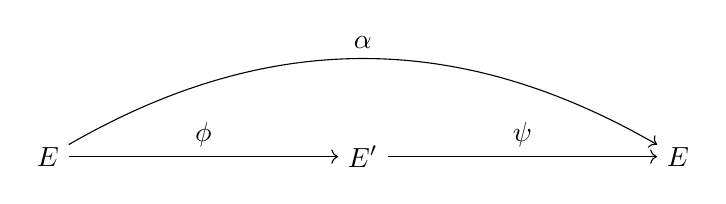
\begin{tikzpicture}
            \node (Ep) at (0, 0) {$E'$};
            \node (E1) at (-4, 0) {$E$};
            \node (E2) at (4, 0) {$E$};

            \draw [->] (E1) -- (Ep) node [midway, above] {$\phi$};
            \draw [->] (Ep) -- (E2) node [midway, above] {$\psi$};
            \draw [->] (E1) to [bend left] node [midway, above] {$\alpha$} (E2);
        \end{tikzpicture}
    \end{center}
    We assume $l \divides n$, otherwise the claim is trivial.
    However, then we have the contradiction
    \begin{align*}
        \psi((\phi \circ \tau \circ \hat{\phi})(P)) &= (\psi \circ \phi \circ \tau \circ \hat{\phi})(P) = (\alpha \circ \tau \circ \hat{\phi})(P) \\
        &= (\tau \circ \alpha \circ \hat{\phi})(P) = (\tau \circ \psi \circ [n])(P) = (\tau \circ \psi)(\IdPoint) = \IdPoint
    \end{align*}
    since $\tau \circ \alpha = \alpha \circ \tau$ ($\End(E)$ is commutative).
\end{proof}
Next, we prove that ideal multiplication is compatible with chaining of isogenies.
Note that the condition $p \notdivides [\O_K : \O]$ is just equivalent to all curves $E$ with $\End(E) \cong \O$ being ordinary.
\begin{lemma}
    Let $\O$ be a quadratic imaginary order with $p \notdivides d(\O)$ with two integral, invertible ideals $\a, \b \leq \O$.
    Let further $E$ be an Elliptic Curve with $\End(E) \cong \O$.
    Identifying $\End(E_\a)$ with $\O$ by the canonical isomorphism $\Phi_{E, \a}: \End(E) \overset{\sim}{\longrightarrow} \End(E_\a)$, we have
    \begin{equation*}
        E_{\a\b} \cong (E_\a)_\b \quad \text{and} \quad \phi_{E, \a\b} = \phi_{E_\a, \b} \circ \phi_{E, \a}
    \end{equation*}
\end{lemma}
\begin{proof}
    First, we show that $\Phi_{E, \a}(\pi_E) = \pi_{E_\a}$ and so we can write $\pi \in \O$ for the unique element mapping to the Frobenius in $\End(E)$ resp. $\End(E_\a)$.
    We have that
    \begin{equation*}
        \Phi_{E, \a}(\pi_E) = \frac 1 {\deg(\phi_{E, \a})} \phi_{E, \a} \circ \pi_E \circ \hat{\phi}_{E, \a}
    \end{equation*}
    and so
    \begin{equation*}
        \phi_{E, \a} \circ \hat{\phi}_{E, \a} \circ \Phi_{E, \a}(\pi_E) = \phi_{E, \a} \circ \pi_E \circ \hat{\phi}_{E, \a}
    \end{equation*}
    Counting separability degrees on both sides shows that $\Phi_{E, \a}(\pi_E)$ is purely inseparable, thus must be the Frobenius $\pi_{E_\a}$.
    
    Now write $\a = \tilde{\a} (p, \pi)^r$ and $\b = \tilde{\b} (p, \pi)^s$.
    It is now the case that
    \begin{equation*}
        \phi_{E, \a\b} = \phi_{E, \tilde{\a} \tilde{\b}}^{(p^{r + s})}
    \end{equation*}
    and
    \begin{equation*}
        \phi_{E_\a, \b} \circ \phi_{E, \a} = (\phi_{E_\a, \tilde{\b}} \circ \pi_r \circ \phi_{E, \tilde{\a}})^{(p^s)} = (\phi_{E_\a, \tilde{\b}} \circ \phi)^{(p^r)} = (\phi_{E_\a, \tilde{\b}}^{(q/p^r)} \circ \phi_{E, \tilde{\a}})^{(p^{r + s})}
    \end{equation*}
    where $\pi_r: E_{\tilde{\a}} \to E_{\tilde{\a}}^{(p^r)}$ is the $p^r$-th power Frobenius and $\phi_{E_\a, \tilde{\b}}$ is defined over $\F_q$.
    Note that $\phi_{E_\a, \tilde{\b}}$ is the separable isogeny with kernel $E_\a[\tilde{\b}]$ and thus $\phi_{E_\a, \tilde{\b}}^{(q/p^r)}$ is the separable isogeny with kernel $E_{\a}^{(q/p^r)}[\tilde{\b}] = E_{\tilde{\a}}[\tilde{\b}]$.
    In other words, find
    \begin{equation*}
        \phi_{E_\a, \tilde{\b}}^{(q/p^r)} = \phi_{E_{\tilde{\a}}, \tilde{\b}}
    \end{equation*}
    and so it suffices to show the claim in the case that $\a = \tilde{\a}$, $\b = \tilde{\b}$ are integral, invertible ideals coprime to $(p, \pi)$.

    Having reduced everything to the separable case, it now suffices to show that $\ker(\phi_{E_\a, \b} \circ \phi_{E, \a}) = E[\a\b]$.
    For simplicity of notation, write $\phi = \phi_{E, \a}$ and $\psi = \phi_{E_\a, \b}$.
    Hence, we want to show that $\ker(\psi \circ \phi) = E[\a\b]$.

    The crucial point here is that our isomorphism $\End(E) \cong \End(E_\a)$ is given by $\Phi$.
    Since the identification of $\End(E)$ and $\End(E_\a)$ would hide this, we will be explicit in this part and write
    \begin{align*}
        i: \O \to \End(E) \quad \text{and} \quad i': \O \to \End(E')
    \end{align*}
    for the isomorphisms.
    Note that $\Phi \circ i = i'$.
    We have
    \begin{align*}
        \ker(\psi \circ \phi) =& \phi^{-1}(\ker\psi) = \phi^{-1}(E'[\mathfrak{a}]) = \phi^{-1}\Bigl( \bigcap_{\tau \in \mathfrak{a}} \ker(i'(\tau)) \Bigr) \\
        =& \bigcap_{\tau \in \mathfrak{a}} \phi^{-1}(\ker(i'(\tau))) = \bigcap_{\tau \in \mathfrak{a}} \ker(i'(\tau) \circ \phi) \overset{(*)}{=} \bigcap_{\tau \in \mathfrak{a}} \ker(\phi \circ i(\tau)) \\
        =& \bigcap_{\tau \in \mathfrak{a}} i(\tau)^{-1}(\ker\phi) = \bigcap_{\tau \in \mathfrak{a}} i(\tau)^{-1}(E[\mathfrak{b}]) = \bigcap_{\tau \in \mathfrak{a}, \ \rho \in \mathfrak{b}} i(\tau)^{-1}(\ker(i(\rho))) \\
        =& \bigcap_{\tau \in \mathfrak{a}, \ \rho \in \mathfrak{b}} \ker(\underbrace{i(\rho) \circ i(\tau)}_{\mathclap{= i(\rho\tau) \in i(\a\b)}}) = E[\mathfrak{b}\mathfrak{a}]
    \end{align*}
    The equality at $(*)$ holds, since
    \begin{equation*}
        i'(\tau) = (\Phi_* \circ i)(\tau) = \frac 1 {\deg(\phi)} \phi \circ i(\tau) \circ \hat{\phi} \qedhere
    \end{equation*}
\end{proof}
The whole reason why the ideal $(p, \pi)$ plays such a special role is that it consists of exactly the inseparable endomorphisms.
\begin{lemma}
    \label{prop:inseparable_iff_frobenius_ideal}
    Let $E$ be an ordinary curve and $\alpha \in \End(E)$.
    Then $\alpha$ inseparable if and only if $\alpha \in (p, \pi)$.
\end{lemma}
\begin{proof}
    First, consider
    \begin{equation*}
        \b := \{ \beta \in \End(E) \ | \ \text{$\beta$ inseparable} \}
    \end{equation*}
    This is an ideal, as for two inseparable $\beta_1, \beta_2 \in \End(E)$ have that they factor as
    \begin{center}
        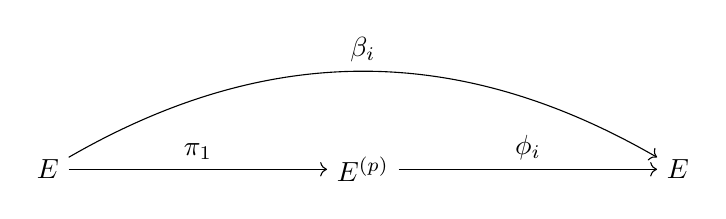
\begin{tikzpicture}
            \node (Ep) at (0, 0) {$E^{(p)}$};
            \node (E1) at (-4, 0) {$E$};
            \node (E2) at (4, 0) {$E$};

            \draw [->] (E1) -- (Ep) node [midway, above] {$\pi_1$};
            \draw [->] (Ep) -- (E2) node [midway, above] {$\phi_i$};
            \draw [->] (E1) to [bend left] node [midway, above] {$\beta_i$} (E2);
        \end{tikzpicture}
    \end{center}
    with the $p$-th power Frobenius $\pi_1$.
    Now $\beta_1 + \beta_2 = (\phi_1 + \phi_2) \circ \pi_1$ is inseparable, and clearly $\beta \gamma$ is inseparable for $\beta \in \b$ and $\gamma \in \End(E)$ (just compare separability degrees).

    Furthermore, $p$ and $\pi$ are inseparable, so $(p, \pi) \subseteq \b$.
    Note that in the imaginary quadratic order $\End(E)$, every prime ideal is maximal.
    Since $\Norm((p, \pi)) = p \perp d(\End(E))$, Prop.~\ref{prop:coprime_ideals_order} shows that $(p, \pi)$ is prime, and thus $(p, \pi) = \b$ (clearly, $\b \neq \End(E)$).
\end{proof}

\begin{lemma}
    Let $E$ be an ordinary curve and $\a, \b \leq \End(E)$ two integral, invertible ideals.
    Then $E_\a \cong E_\b$ if and only if $[\a] = [\b] \in \Cl(\End(E))$ are in the same ideal class.
\end{lemma}
\begin{proof}
    First, we show the direction $\Leftarrow$.
    By assumption, there are $\alpha, \beta \in \O$ such that $\alpha\a = \beta\b$.
    Thus $E_{\alpha\a} = E_{\beta\b}$ and it suffices to show that for any Elliptic Curve $E$ and $\alpha \in \End(E)$, have $E_{(\alpha)} \cong E$.

    Write $(\alpha) = (p, \pi)^r \a$ and assume that $E$ is defined over $\F_{p^s}$.
    Then $(\alpha)(p)^{\lceil r/s \rceil s - r} = (\pi)^{\lceil r/s \rceil}(\alpha')$ since $(p) = (p, \pi)(p, \pi - t)$ and $(p, \pi)^s = (\pi)$ by an easy computation.
    Furthermore, $\alpha' \notin (p, \pi)$.
    Now note that for any curve $E$, have $E_{(\pi)} = E^{(p^s)} \cong E$ and $E_{(p)} \cong E$, where the latter holds, since in the ordinary case, $p$ factors as
    \begin{center}
        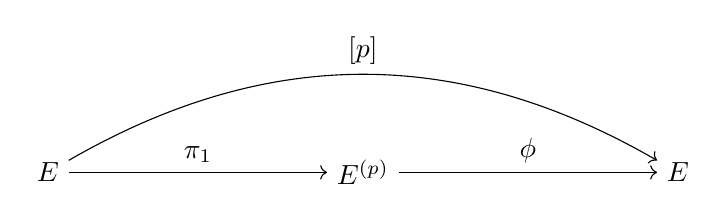
\begin{tikzpicture}
            \node (Ep) at (0, 0) {$E^{(p)}$};
            \node (E1) at (-4, 0) {$E$};
            \node (E2) at (4, 0) {$E$};

            \draw [->] (E1) -- (Ep) node [midway, above] {$\pi_1$};
            \draw [->] (Ep) -- (E2) node [midway, above] {$\phi$};
            \draw [->] (E1) to [bend left] node [midway, above] {$[p]$} (E2);
        \end{tikzpicture}
    \end{center}
    with the $p$-th power Frobenius $\pi_1$ and $\phi$ is separable with $\ker(\phi) = E[p] = \ker([p]) \cap \ker(\pi - t)$.
    Thus we see that $E_{(\alpha)} \cong E_{(\alpha')}$ and can assume wlog that $\alpha = \alpha' \notin (p, \pi)$.

    By Lemma~\ref{prop:inseparable_iff_frobenius_ideal}, we now see that $\alpha$ is separable, and so clearly $\ker(\alpha) = E[(\alpha)]$.
    Since $\alpha: E \to E$ is the separable isogeny on $E$ with kernel $E[(\alpha)]$, we see that $E_{(\alpha)} = E/E[(\alpha)] \cong E$.

    Now we consider the other direction $\Rightarrow$.
    Again, write $\a = \tilde{\a}(p, \pi)^r$ and assume that $E$ is defined over $\F_{p^s}$.
    Then we have as before that $\a (p)^{\lceil r/s \rceil s - r} = (\pi)^{\lceil r/s \rceil} \a'$ for the ideal $\a' = \tilde{\a} (p, \pi - t)^{\lceil r/s \rceil s - r}$.
    Now clearly $[\a] = [\a']$ are in the same ideal class and $\a' \perp (p, \pi)$.
    Furthermore, by the direction $\Leftarrow$, have $E_\a \cong E_{\a'}$.
    Doing the same with $\b$, we can assume wlog that $\a = \a'$ and $\b = \b'$ are ideals coprime to $(p, \pi)$.

    Therefore, the isogenies $\phi_{E, \a}$ and $\phi_{E, \b}$ are separable.
    Write $E' := E_\a = E_\b$.
    Choose $N > 0$ such that $[N]^{-1}(E[\a]) \supseteq E[\b]$.
    Now the isogeny $[N] \circ \phi_{E, \a}$ factors through $\phi_{E, \b}$, i.e. we get a commutative diagram
    \begin{center}
        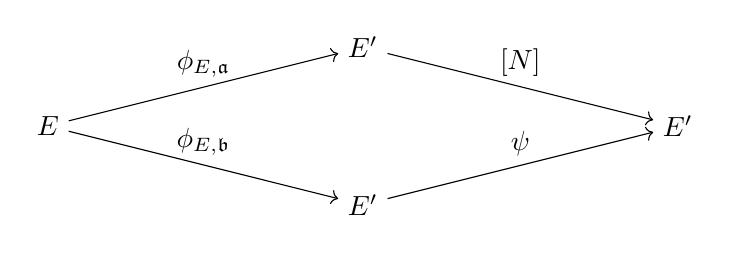
\begin{tikzpicture}
            \node (E1) at (0, 1) {$E'$};
            \node (E2) at (0, -1) {$E'$};
            \node (E0) at (-4, 0) {$E$};
            \node (E3) at (4, 0) {$E'$};

            \draw [->] (E0) -- (E1) node [midway, above] {$\phi_{E, \a}$};
            \draw [->] (E0) -- (E2) node [midway, above] {$\phi_{E, \b}$};
            \draw [->] (E1) -- (E3) node [midway, above] {$[N]$};
            \draw [->] (E2) -- (E3) node [midway, above] {$\psi$};
        \end{tikzpicture}
    \end{center}
    for some endomorphism $\psi: E' \to E'$.
    Clearly the isogenies $[N]$ and $\psi$ are given by the ideals $(N)$ resp. $(\psi)$, and so we find
    \begin{equation*}
        (N)\a = (\psi)\b
    \end{equation*}
    and the claim follows.
\end{proof}
Now we have proven almost everything we need.
The final ingredient, from which it will then follow that the class group action is transitive, is a theorem of Tate.
Since it uses much of the theory on general abelian varieties, we will present it without proof here.
For a proof, the reader is referred to the work of Tate \cite{tate}.
\begin{theorem}[Isogeny theorem]
    \label{prop:isogeny_theorem}
    Let $E$, $E'$ be Elliptic Curves defined over $\F_q$.
    Then there is a separable isogeny $E \to E'$ if and only if $\#E(\F_q) = \#E'(\F_q)$.
\end{theorem}
Note that this condition is also equivalent to $\End(E) \otimes \Q \cong \End(E') \otimes \Q$ or that the $q$-th power Frobenius endomorphisms have the same trace. 
\begin{theorem}
    \label{prop:class_group_action}
    Let $\O$ be an imaginary quadratic order with $p \notdivides d(\O)$ and denote by $\Ell(\O)$ the set of isomorphism classes of all Elliptic Curves $E$ over $\bar{\F}_p$ with $\End(E) \cong \O$.
    Then there is a free and transitive group action
    \begin{equation*}
        \Cl(\O) \times \Ell(\O) \to \Ell(\O), \quad ([\a], E) \mapsto E_\a
    \end{equation*}
    where $\a$ is an integral, invertible ideal representative of the ideal class $[\a]$.
\end{theorem}
\begin{proof}
    Well-definedness and freeness follow from all the previous lemmas.
    So it is left to derive the transitivity from Thm~\ref{prop:isogeny_theorem}.
    Let $E$ and $E'$ be curves in $\Ell(\O)$.
    Clearly, we then have $\#E(\F_q) = \#E'(\F_q)$ and so there is a separable isogeny $\phi: E \to E'$.
    Everything we have to show is that $\phi = \phi_{E, \a}$ for some ideal $\a \leq \O$.
    \\\\TODO
\end{proof}
A similar class group action exists in many other cases, since it is really founded in the theory of abelian varieties, see \cite{class_group_action_waterhouse}.
Notable examples are the CSIDH class group action for supersingular curves defined over $\F_p$ (see \cite{csidh}), its generalization to so-called oriented curves (see \cite{osidh}), and the very classical class group action of Elliptic Curves with complex multiplication (over $\C$).
More concretely, if we consider an order $\O$ in a quadratic imaginary number field and write $\Ell(\O)$ for the set of (isomorphism classes of) curves over $\C$ with endomorphism ring $\O$ (these are said to have \emph{complex multiplication}), then there is a free and transitive class group action
\begin{equation*}
    \Cl(\O) \times \Ell(\O) \to \Ell(\O), \quad ([\a], E) \to E/E[\a]
\end{equation*}
where we choose $\a$ to be an integral ideal representative of $[\a]$.
Note that for ideals $\a \perp (p, \pi)$, this is analogous to our action defined above.
However, since the Frobenius has trivial kernel, one needs some addition in the finite field case.

Note that one can still keep the simpler definition
\begin{equation*}
    \Cl(\O) \times \Ell(\O) \to \Ell(\O), \quad ([\a], E) \to E/E[\a]
\end{equation*}
also in the finite field case, if we require $\a$ to be an (integral) ideal representative of $[\a]$ that is coprime to $(p, \pi)$.
Clearly, every ideal class has such a representative, since we can multiply with the principal ideal $(p) = (p, \pi)(p, \pi - t)$ and divide out the principal ideal $(\pi) = (p, \pi)^s$.
However, some sources do not explicitly mention that $\a$ must be chosen coprime to $(p, \pi)$, which caused me some confusion.

\subsection{Vulcanos}
Once we have the class group action, we can derive a lot of information about the structure of the ordinary part of an isogeny graph.
\begin{definition}
    Denote by $\Gamma_l(\F_q)$ the graph whose vertices are isomorphism classes of Elliptic Curves over $\F_q$, and the edges are the degree $l$ isogenies between them (with multiplicity).
\end{definition}
Since there is never an isogeny between ordinary and supersingular curves, we will continue to talk of ordinary and supersingular connected components of $\Gamma_l(\F_q)$.
Note that by the j-invariant, an isomorphism class of an Elliptic Curve $E$ is in 1-to-1 correspondence with the j-invariant $j(E)$, and so we could also say that the vertices of $\Gamma_l(\F_q)$ are just the elements of $\F_q$.
Furthermore that the existence of the dual isogeny implies that $\Gamma_l(\F_q)$ is undirected.
\begin{definition}
    For $l > 0, d \geq 0$, a graph $G$ is called \emph{$l$-vulcano of depth $d$}, if its vertices can be partitioned into a set $C$ (the ``crater'') and a set $L$ (the ``lava flows'') such that
    \begin{itemize}
        \item $G[C]$ is either a single vertex (possibly with one or two loops), two connected vertices or a cycle of at least two vertices\footnote{A cycle of two vertices shall be two vertices with a double edge.}
        \item $G[V]$ is a forest of complete $l$-ary trees of depth $d$
        \item Every vertex $v \in C$ is connected to the roots of $l + 1 - \deg_{G[C]}(v)$ trees in $G[V]$
    \end{itemize}
    In particular, every vertex in $G$ except the leaves of the trees has degree $l + 1$.
\end{definition}
The term ``vulcano'' was introduced by \cite{isogeny_vulcano}, after Kohel had mostly determined the structure of ordinary connected components in his PhD thesis.
Most of this follows from the above class group action, and for the remaining details we refer the reader to Kohel's thesis \cite[Prop.~23]{kohel}.
\begin{theorem}
    \label{prop:isogeny_vulcano}
    Let $G$ be a connected component of $\Gamma_l(\F_q)$.
    Suppose that $G$ is ordinary, i.e. its vertices are (isomorphism classes of) ordinary curves.
    Then $G$ is an $l$-vulcano.
    Further, we have
    \begin{itemize}
        \item All curves on the crater have the same endomorphism ring $\O$ with $l \notdivides [\O_{\O \otimes \Q} : \O]$.
        \item All curves on the $i$-th tree level of a lava flow have the endomorphism ring $\Z + l^i\O$.
        \item The size of the crater is the order of $\l_1$ in $\Cl(\O)$, where $(l) = \l_1\l_2$ in $\O$, or 1 if $l$ is inert in $\O$.
    \end{itemize} 
\end{theorem}

\section{The supersingular case}
\label{sec:supersingular_isogeny_graph}
After studying the ordinary connected components of the $l$-isogeny graph $\Gamma_l(\F_q)$, we now come to the supersingular component(s).
First, note that all supersingular j-invariants are defined over $\F_{p^2}$, and so we will assume $q = p^2$ for this section.

In the supersingular setting, the endomorphism ring is now non-commutative.
There still exists a non-commutative analogue of the class group action, but using that structure is significantly harder.
Mainly, because the theory of quaternion algebras is more complicated, and its class group structure is less studied.

Instead, there is the famous result of Pizer, which states that supersingular isogeny graphs (i.e. the supersingular part of $\Gamma_l(\F_q)$) are so called Ramajuan graphs, that is have excellent expander properties.
We will introduce this result in this section, but without proof.
\begin{definition}
    \label{def:expander}
    A $d$-regular graph $G$ is called $\epsilon$-expander, if the eigenvalues $\lambda_1 > ... > \lambda_n$ of its adjacency matrix satisfy
    \begin{equation*}
        |\lambda_2|, |\lambda_n| \leq (1 - \epsilon) d
    \end{equation*}
\end{definition}
In the literature, expander graphs are often defined by the use of the expansion ration
\begin{equation*}
    h(G) := \min_{S \subseteq V, \ \#S \leq \frac n 2} \frac {\#\partial S} {\# S}
\end{equation*}
of a graph $G = (V, E)$.
Here $\partial S$ is the edge boundary, i.e. the set of edges between a point in $S$ and a point in $V \setminus S$.

The connection between those two definitions is then given by the Cheeger-inequality
\begin{prop}
    Let $G$ be a $d$-regular graph such that its adjacency matrix has eigenvalues $\lambda_1 > ... > \lambda_n$.
    Then
    \begin{equation*}
        \frac {d - \lambda_2} 2 \leq h(G) \leq \sqrt{2d(d - \lambda_2)}
    \end{equation*}
\end{prop}
\begin{proof}
    See e.g. \cite{cheeger_inequality}.
\end{proof}
This inequality only correlates the so-called spectral gap $d - \lambda_2$ with $h(G)$, and does not bound $|\lambda_2|$.
In many cases, bounds on the spectral gap or expansion ration already suffice to show properties of expanders.
Because of this, expanders are usually defined as graphs for which $\lambda_2$ or $h(G)$ are bounded.
Our definition~\ref{def:expander} is then sometimes called ``two-sided expander''.
However, we will never use one-sided expanders in this work, hence the above definition shall be sufficient.

The nice thing about the expansion ratio is that it gives more intuition on what the expander property means.
In particular, an expander graph is densely connected, i.e. by deleting a small number of edges, it is impossible to make the graph split into two (or more) connected components of relatively large size.
\begin{definition}
    A connected $d$-regular graph is called Ramajuan, if
    \begin{equation*}
        |\lambda_2|, |\lambda_n| \leq 2\sqrt{d - 1}
    \end{equation*}
    where $\lambda_1 > ... > \lambda_n$ are again the eigenvalues of the adjacency matrix.
\end{definition}
It is known that the bound $2\sqrt{d - 1}$ is asymptotically optimal, i.e. for sufficiently large $n$, all $d$-regular graphs of $n$ vertices have $\lambda_2 \geq 2\sqrt{d - 1} - \epsilon$.
In that sense, we can say Ramajuan graphs are graphs with asymptotically optimal expansion properties.

One of the main properties of expander graphs is random walks on them mix rapidly.
That is, the final vertex of relatively short random walks is distributed almost uniformly among all vertices.
\begin{theorem}
    \label{prop:expander_random_walk}
    Let $G = (V, E)$ be a $d$-regular $\epsilon$-expander graph and $v \in V$ a vertex.
    Then the distribution of the final vertex of a random walk starting from $v$ of length $t$ is close to uniform, in particular, the $\ell_2$-statistical distance is bounded by $(1 - \epsilon)^t$.
\end{theorem}
For a proof of this theorem, see e.g. Thm~3.3 in this excellent survey on expander graphs \cite{expander_survey}.
Note that expander graphs used in cryptography are usually of exponential size, so this theorem says that a random walk of polynomial length already reaches all vertices of the graph.

Now we come to the anticipated result, that supersingular isogeny graphs are expander graphs.
\begin{definition}
    The \emph{supersingular $l$-isogeny graph over $\F_{p^2}$} is the subgraph of $\Gamma_l(\F_{p^2})$ induced by all (isomorphism classes of) supersingular curves over $\F_{p^2}$.
\end{definition}
Since the supersingular $l$-isogeny graph is disconnected from the rest of $\Gamma_l(\F_{p^2})$, we see that it is an $(l + 1)$-regular graph.
We also know its size exactly, which directly follows from a classical result on the number of supersingular curves over $\F_{p^2}$.
\begin{prop}
    For $p \geq 5$, there are exactly
    \begin{equation*}
        \left\lfloor \frac p {12} \right\rfloor + \begin{cases}
            0 & \text{if $p \equiv 1 \mod 12$} \\
            1 & \text{if $p \equiv 5, 7 \mod 12$} \\
            2 & \text{if $p \equiv 11 \mod 12$}
        \end{cases}
    \end{equation*}
    supersingular Elliptic Curves over $\F_{p^2}$.
\end{prop}
For a proof of this statement, see e.g. \cite[Thm~V.4.1]{arithmetic_elliptic_curves}.

In \cite{supersingular_graphs_ramajuan}, Pizer has now shown that
\begin{theorem}
    \label{prop:supersingular_graph_ramajuan}
    The supersingular $l$-isogeny graph is Ramajuan.
\end{theorem}
This shows that there is a huge difference between the ordinary and supersingular graphs.
For example, there is always a path of length $O(\log(p))$ between two curves in the supersingular graph, but in the ordinary graph, such a path does not exist in many cases.
We will try to quantify this in the last section.
The idea of our research is to utilize these differences in order to find random, supersingular curves.

\section{Modular polynomials}
If we want to work computationally with isogeny graphs, we need a way to explicitly compute them.
The simplest way to find the $m$-isogeny neighbors of a curve $E$ is to compute $E[m]$ and find the order-$m$-subgroups.
While this works in many cases, it can happen that the torsion group $E[m]$ only lies in an extension of $\F_q$ of degree $O(m^2)$, in which it is very costly to work.
Furthermore, there are many other applications where a torsion-based approach does not work at all.

In the ordinary case, the class group action might be also used to compute neighbors in the $l$-isogeny graph, provided we know the endomorphism ring of the start curve.
However, finding the endomorphism ring is a hard problem in itself, and thus this method is not really practical.
Furthermore, this does not work in the supersingular setting.

One solution to this problem is given by modular curves, which give a very useful algebraic structure to the $l$-isogeny graph.
In particular, the existence of a nontrivial $l$-isogeny between curves is an algebraically closed condition, i.e. is given by an algebraic curve.

The classical way to study this is by using the theory of modular forms.
Since this is out of the scope of this work, we refer to \cite[§11]{cox_primes_of_form} for an introduction of the topic.
The basic result is the following.
\begin{theorem}
    \label{prop:complex_mod_poly}
    For $m \geq 2$ there is an irreducible and monic polynomial
    \begin{equation*}
        \Phi_m(X, Y) \in \Z[X, Y]
    \end{equation*}
    such that for Elliptic Curves $E, E'$ defined over $\C$, there is a cyclic $m$-isogeny $E \to E'$ if and only if $\Phi_m(j(E), j(E')) = 0$.
\end{theorem}
This polynomial is called the \emph{(classical) modular polynomial of level $m$}.
A proof of this theorem is e.g. given in \cite[Thm~11.18]{cox_primes_of_form}.
A few corollaries of this theorem can easily be inferred.
\begin{corollary}
    Let $m \geq 2$. Then we have
    \begin{itemize}
        \item $\Phi_m$ is symmetric, i.e. $\Phi_m(X, Y) = \Phi_m(Y, X)$.
        \item $\Phi_m$ has degree $\psi(m)$ (as polynomial in $X$), where $\psi$ is the Dedekind $\psi$-function
        \begin{equation*}
            \psi(m) = m \prod_{p \divides m} 1 + \frac 1 p
        \end{equation*}
    \end{itemize}
\end{corollary}
\begin{proof}
    The first statement follows from the existence of the dual isogeny.
    For the second statement, note that for each Elliptic Curve $E$ over $\C$, the degree of $\Phi_m(X, j(E))$ is the number of curves $E'$ with an $m$-isogeny $E \to E'$, which is equal to the number of cyclic subgroups $G \leq E \cong (\mathbb{R}/\Z)^2$ of size $m$.
    By the Chinese Remainder theorem, this is a multiplicative function, and for a prime power $m = p^k$, the number is
    \begin{align*}
       &\#\bigl\{ G \leq (\Z/m\Z)^2 \ \bigm| \ \#G = m \bigr\} \\
       =& \#\bigl\{ \langle (1, \alpha) \rangle \ \bigm| \ \alpha \in \Z/m\Z \bigr\} + \#\bigl\{ \langle (\alpha, 1) \rangle \ \bigm| \ \alpha \in (\Z/m\Z) \setminus (\Z/m\Z)^* \bigr\} \\
       =& p^k + \#\bigl\{ \langle (\alpha, 1) \rangle \ \bigm| \ \alpha \in p(\Z/m\Z) \bigr\} = p^k + p^{k - 1} \\
       =& m \left( 1 + \frac 1 p \right) \qedhere
    \end{align*}
\end{proof}
Since we are mainly interested in the case of finite fields, we have to show that the modular polynomial behaves well under reductions mod $p$.
First, we use two lemmas.
\begin{lemma}
    \label{prop:modified_hensel_lifting}
    Let $f \in \O_K[X]$ be a polynomial for some number field $K$ with a prime $\p$.
    If $f(X) \mod \p \in \F_q[X]$ has a root $\alpha$, then $f$ has a root in $\O_L$ that reduces to $\alpha$ modulo a prime over $\p$ for some finite field extension $L/K$.
\end{lemma}
\begin{proof}
    Follows by Hensel's Lemma.
\end{proof}
\begin{lemma}
    Let $E$ and $E'$ be curves over $\F_q$ and $\phi: E \to E'$ a cyclic $m$-isogeny.
    Then there exist curves $E_0$, $E_0'$ with j-invariant in $\O_K$ for some number field $K$ with a prime $\p$ over $p = \mathrm{char}(K)$ and an isogeny $\phi_0: E_0 \to E_0'$ such that
    \begin{equation*}
        \tilde{E}_0 = E, \ \tilde{E}_0' = E' \quad \text{and} \quad \tilde{\phi}_0 = \phi
    \end{equation*}
    where $\tilde{\cdot}$ is the reduction modulo $\p$.
\end{lemma}
\begin{proof}
    Consider some arbitrary lift $E_0$ and $E_0'$ of $E$ resp. $E'$ to a number field $K$ such that $j(E_0), j(E_0') \in \O_K$.
    Assume that $E_0'$ is defined by a homogeneous polynomial $f = Y^2Z - X^3 - AXZ^2 - BZ^3 \in \O_K[X, Y, Z]$.
    Finally, assume $\phi = [u : Y v : w]$ with polynomials $u, v, w \in \F_q[X]$ and choose an arbitrary lift $v_0, w_0 \in \O_K[X]$ of $v$ resp. $w$.
    Hence the coefficients $u^{(0)}, ..., u^{(n)}$ of $u \in \F_q[X]$ are a root of
    \begin{equation*}
        f(\sum T_i X^i, Y v_0, w_0) = \sum_i a_i(T_0, ..., T_n) X^i \in \O_K[X][T_i]
    \end{equation*}
    modulo $\p$.
    Note that the coefficient of $X^j$ in $(\sum_i T_i X^i)^3$ contains the monomial $T_0^2 T_j$, and wlog we have chosen the lifts of $A, B$ such that also the coefficient in $f(\sum T_i X^i, Y v, w)$ does.
    Furthermore, the coefficient of $X^j$ in $f(\sum T_i x^i, Y v, w)$ is in $\O_K[T_0, ..., T_j]$, i.e. only depends on $T_0, ..., T_j$.

    wlog $u_0 \neq 0$, otherwise we can just move $E'$ in $x$-direction by some element in $\p$, which preserves $\tilde{E}_0' = E'$.

    Now Lemma~\ref{prop:modified_hensel_lifting} shows that there is a lift $u^{(0)}_0$ of $u^{(0)}$ in some number field $L_0/K$ with $a_0(u^{(0)}_0) = 0$.
    Since $u_0^{(0)} \neq 0$, we see that $a_i(u_0^{(0)}, ..., u_0^{(i - 1)}, T_i)$ contains the monomial $T_i$, and so applying the lemma inductively, we also find lifts $u^{(1)}_0, ..., u^{(d)}_0 \in \O_L/K$ with $a_i(u^{(0)}_0, ..., u^{(i)}_0) = 0$, where $d = \deg(u)$.
    In other words, we found a lift $u_0$ of $u$ in $\O_L[X]$ such that $f(u_0, Y v_0, w) = 0$.
    Now we can set $\phi_0 = [u_0 : Y v_0 : w_0]: E_0 \to E_0'$ and the claim follows.
\end{proof}
Using more Hensel lifting, we now can pull down the properties of $\Phi_m$ to finite fields.
\begin{prop}
    For $m \geq 2$ and Elliptic Curves $E$ and $E'$ over $\F_q$, have $\Phi_m(j(E), j(E')) = 0 \in \F_q$ if and only if there is a cyclic $m$-isogeny $E \to E'$.
\end{prop}
\begin{proof}
    First, consider the direction $\Leftarrow$.
    Here the previous Lemma shows that we can lift the situation to $m$-isogeneous curves $E_0$ and $E_0'$ over a number field $K$, and so have by Prop.~\ref{prop:complex_mod_poly} that
    \begin{equation*}
        \Phi_m(j(E_0), j(E_0')) = 0
    \end{equation*}
    Furthermore we know that $j(E_0), j(E_0') \in \O_K$, and so we clearly have for the reduction modulo $\p$ that
    \begin{equation*}
        \Phi_m(j(E), j(E')) \equiv \Phi_m(j(E_0), j(E_0')) \equiv 0 \mod \p
    \end{equation*}

    Now we show the direction $\Rightarrow$.
    We have $\Phi_m(j(E), j(E')) = 0 \in \F_q$, thus there is a number field $K$ with a prime $\p$ over $p = \mathrm{char}(\F_q)$ and $x, y \in \O_K$ such that
    \begin{equation*}
        \Phi_m(x, y) \equiv 0 \mod \p \quad \text{and} \quad x \equiv j(E), \ y \equiv j(E') \mod \p
    \end{equation*}
    Now we can again use Lemma~\ref{prop:modified_hensel_lifting} to find $x'$ in the completion $K_\p$ such that $x' \equiv x \mod \p$ and $\Phi_m(x', y) = 0 \in K_\p$.
    Since $x'$ is a root of $\Phi_m(X, y)$, it is algebraic and thus an algebraic integer.
    So there is a number field $K'$ with a prime $\p'$ over $\p$ such that $x', y \in K'$ and $x' \equiv j(E)$, $y \equiv j(E')$ modulo $\p'$.
    In particular, there are curves $E$, $E'$ over $K'$ with j-invariants $x'$ resp. $y$, and thus by Prop.~\ref{prop:complex_mod_poly}, there is a cyclic $m$-isogeny $E \to E'$.
    Therefore, there is also an $m$-isogeny between the curves $\tilde{E}$ and $\tilde{E}'$, which are the reductions of $E$ resp. $E'$ modulo $\p'$.
\end{proof}
Some properties however do not holds anymore.
For example, in the finite field case, $\Phi_m$ might not be irreducible anymore.
In fact, it is easy to see that
\begin{equation*}
    \Phi_p(X, Y) \equiv -(X^p - Y)(Y^p - X) \mod p
\end{equation*}
since the only $p$-isogenies over a field of characteristic $p$ are the Frobenius and its conjugate.

The modular polynomial is an indispensable tool when doing computations on the isogeny graph.
In particular, when combined with an algorithm to factor polynomials over $\F_q$, it allows us to compute all the neighbors of a curve $E$ in the $l$-isogeny graph.
For example Sutherland's supersingular test \cite{sutherland_supersingularity_test} uses modular polynomials for walks in the isogeny graph, and distinguishes ordinary and supersingular curves by the structure of their isogeny graph neighborhoods.
Another example is Shoof's algorithm \cite{shoof_point_counting} for counting $\F_q$-rational points on a curve, which also fundamentally relies on modular polynomials.

Therefore, computing modular polynomials is an important task.
The most classical approach is to mimic to proof of Thm~\ref{prop:complex_mod_poly}, i.e. view Elliptic Curves as lattices over $\C$ and compute the Fourier coefficients of the $j$-function.
However, one main problem is that the coefficients in the modular polynomial become very large very fast.
For example, $\Phi_5$ has already the constant coefficient
\begin{equation*}
    141359947154721358697753474691071362751004672000
\end{equation*}
In many cases, we only need the value of $\Phi_m$ modulo a prime $p$, and thus other algorithms can easily be faster.
A whole line of work tries to use isogeny graphs over finite fields to find such an algorithm, see e.g. \cite{compute_modular_polynomial} and \cite{compute_modular_polynomial2}.
Using the Chinese Remainder theorem, these algorithms can also be used to find $\Phi_m$ over $\C$ by collecting information modulo many different primes.


\chapter{Generating supersingular curves}


Since the advent of the SIDH scheme \cite{sidh}, supersingular curves are at the center of attention in isogeny-based cryptography.
The most important hard problem in that context is the \emph{(supersingular) isogeny path problem}, defined as finding an isogeny of smooth degree (or sometimes power-$l$ degree) between two given supersingular curves.
This problem is also equivalent \cite{endomorphism_ring_reductions} to the supersingular endomorphism ring problem, that is to compute a basis of the endomorphism ring of a supersingular curve.
In many cryptographic application, it is helpful or even required that supersingular curves used to instantiate the scheme do not come with a trapdoor that might simplify solving one of these problems.
More concretely, we want to instantiate the scheme with a random supersingular curve, for which nobody knows the endomorphism ring or a smooth isogeny to a previously fixed curve.
Hence it is an important question how we can compute a random supersingular curve in a way that the computation does not reveal such information - or more precisely, that it is impossible to efficiently compute this information given the randomness used for finding the curve. 

Up to now, the only attempt at solving this problem is in \cite{base_paper}, who proposed several highly interesting ideas.
However, each of them currently has some major obstacle that must be overcome before one can get a practical method.
Three of the five presented ideas are based on defining polynomial systems whose roots are (overwhelmingly) supersingular, and then try to find a random root of the system.
The main problem with those methods is that the considered polynomials are too large to work with efficiently.
Furthermore, current tools to solve polynomial systems like resultants and in particular Groebner bases are often impractical even for moderately sized inputs.

Our research focused on the second idea of \cite{base_paper}, which is based on modular polynomials.
We found answers to some of the questions in the paper, as well as a variation of the method that has properties that might help with efficiently computing it.
However, the algorithm is still not practical.
In this chapter, we present those results, after first discussing some naive approaches.

\section{Naive approaches}
First, we have a look at some simple approaches to the problem, to get a feeling for the challenges.

\paragraph{Random Sampling} It is a folklore knowledge that all supersingular curves over $\bar{\F}_p$ have a j-invariant in $\F_{p^2}$, i.e. are isomorphic to a curve defined over $\F_{p^2}$.
Hence, the most naive approach is to sample random $j \in \F_{p^2}$ and check if they define supersingular curves.
It is clear that this algorithm does not reveal any information about isogenies or the endomorphism ring of the found curve, unless the information can be efficiently computed from the curve itself (in which case the cryptographic schemes are broken anyway).
However, the number of supersingular curves over $\F_{p^2}$ is only approximately $p/12$, which means that the expected number of required samples (and supersingularity checks) is about $12p$, which is exponential in $\log(p)$.

\paragraph{Random Walk} Opposed to that we have the way supersingular curves are currently generated:
As discussed in Section~\ref{sec:supersingular_isogeny_graph}, a random walk of length polynomial in $\log(p)$ in the supersingular $l$-isogeny graph is sufficient to find an (almost) uniformly distributed supersingular curve.
As long as we know one fixed curve to start with, this is quite efficient.
However, clearly this computation reveals a power-$l$ degree isogeny to the fixed starting curve, which is exactly what we want to avoid.

\paragraph{Polynomial with supersingular roots} An idea that is more similar to what we will do next, is to use the following theorem from \cite[Thm~V.4.1]{arithmetic_elliptic_curves}.
\begin{theorem}
    Let $p$ be an odd prime and $m = (p - 1)/2$. Then the Elliptic Curve given by $y^2 = x(x - 1)(x - \lambda)$ over $\F_q$ is supersingular, if and only if
    \begin{equation*}
        H_p(\lambda) := \sum_{i = 0}^m {m \choose i}^2 \lambda^i = 0
    \end{equation*}
\end{theorem}
In other words, we just have to find a random root of the polynomial $H_p(X)$, which then gives rise to a random supersingular curve.
The obvious problem here is again that $p$ is exponential in the input size $\log(p)$, thus the polynomial $H_p(X)$ also has exponential degree, and it is not clear if we can find a random root efficiently.
In fact, the first idea in \cite{base_paper} is use a method similar to the Newton-Raphson algorithm to find a random root.
However, that seems to be only moderately successful.

\section{GCDs of modular polynomials}
The second idea of \cite{base_paper}, which we want to study in more detail, is based on the following intuition:

Since the supersingular isogeny graph is an expander, it is relatively likely that there is an $n$-isogeny between two random curves $E$ and $E'$ (for a fixed $n$).
On the other hand, this is much less likely in the ordinary case.
We expect that this still applies when we take not two random curves, but a random curve $E$ and its Frobenius conjugate $E^{(p)}$, i.e. the curve with j-invariant $j(E)^p$.
Hence, the roots of
\begin{equation*}
    \Phi_n(X, X^p)
\end{equation*}
should contain a relatively large fraction of supersingular roots over $\F_{p^2}$.
More concretely, from the OSDIH class group action, see e.g. \cite[Thm~4.3]{chenu_smith}, we can derive the following corollary.
\begin{corollary}
    \label{prop:osidh_class_group_action}
    There are $\Theta(\sqrt{mp})$ supersingular curves $E$ over $\F_{p^2}$ with an $m$-isogeny to $E^{(p)}$.
\end{corollary}
Since it has degree $np$, it has in total $np$ roots in $\bar{\F}_p$, which means that the fraction of supersingular roots is still exponentially small.
Of course, it might be more interesting to find the number of roots over $\F_{p^2}$, but this turns out to be somewhat tricky.
Another obvious problem with this polynomial is that it has exponential degree, so it is not clear how to compute its roots.

To tackle these two problems, \cite{base_paper} proposed to instead take the polynomial
\begin{equation*}
    f_{p, n, m} = \gcd(\Phi_n(X, X^p), \Phi_m(X, X^m))
\end{equation*}
The idea to find a root of this is to take a non-square $d \in \F_p$ and its square root $\delta \in \F_{p^2}$.
Then $(a + b\delta)^p = a - b\delta$ and so we can equivalently look for $x, y \in \F_p$ such that
\begin{equation*}
    \Phi_n(x + \delta y, x - \delta y) = \Phi_m(x + \delta y, x - \delta y) = 0
\end{equation*}
Hence, we look for a root in $\F_p$ of the polynomial
\begin{equation*}
    \mathrm{res}_Y(\Phi_n(X + \delta Y, X - \delta Y), \Phi_m(X + \delta Y, X - \delta Y))
\end{equation*}
However, note that a solution to this system will have an endomorphism of degree $nm$.
If we choose both $n$ and $m$ of size polynomial in $\log(p)$, this means the endomorphism ring has polynomial discriminant, which is a weakness (in particular, there are only polynomially many curves with such an endomorphism ring).
Hence, at least one of $n$ resp. $m$ has to be of super-polynomial (or better exponential) degree in $\log(p)$.

This of course makes it very hard to even write down or compute some properties of $\Phi_n$.
Hence, we will study a slight modification and focus on the case that $n = l^e$ is a prime power.

\subsection{The prime power case}
First of all, we describe how the assumption $n = l^e$ might help us to work with $\Phi_n$.
Note that $\Phi_{l^e}(j(E), j(E'))$ is equivalent to there being a cyclic $l^e$-isogeny between $E$ and $E'$.
If we relax this to just any $l^e$-isogeny and note that an $l^e$-isogeny is equal to an $l$-isogeny path of length $e$, we can instead work with the condition
\begin{equation*}
    \exists x_1, ..., x_{e - 1}: \ \Phi_l(x, x_1) = \Phi_l(x_1, x_2) = ... = \Phi_l(x_{e - 1}, y)
\end{equation*}
In other words, we look for a solution to the polynomial system
\begin{equation*}
    F_{p, m, l^e} := \langle \Phi_m(x, y), \Phi_l(x, x_1), ..., \Phi_l(x_{e - 1}, y) \rangle
\end{equation*}
The other advantage of this approach is that every supersingular curve $E$ has an $l^e$-isogeny to $E^{(p)}$ if $e \geq O(\log_l(p))$.
This follows from our results on expander graphs.
More concretely, Thm~\ref{prop:supersingular_graph_ramajuan} shows that the supersingular $l$-isogeny graph over $\F_{p^2}$ is an $\epsilon$-expander for
\begin{equation*}
    \epsilon = 1 - \frac {2\sqrt{d - 1}} d = 1 - 2 \frac {\sqrt{l}} {l + 1} \geq 1 - \frac 2 {\sqrt{l}}
\end{equation*}
Thus, a random walk of length at least
\begin{equation*}
    -\log_{2/\sqrt{l}}(p/12) = O(\log_l(p))
\end{equation*}
has a nonzero probability of ending in any fixed vertex, by Thm~\ref{prop:expander_random_walk}.
Note further that for moderately large $l$, the constant approaches $2$, i.e. we can choose $e \approx 2\log_l(p)$.

This leaves us with a polynomial system of $O(\log(p))$ unknowns and equations, which at least can be explicitly written down.
Now we want to study how big the fraction of supersingular roots is.
However, since by our choice of $e = \Theta(\log_l(p))$, we can assume that all supersingular j-invariants are roots of $\Phi_{l^e}(X, X^p)$, and so the number of supersingular roots is $O(\sqrt{mp})$, again by Corollary~\ref{prop:osidh_class_group_action}.
Hence, we want to find instances of $l, e$ and $m$ such that above system has at most $O(\mathrm{poly}(\log(p)))$ ordinary roots. 

\subsection{Studying the number of ordinary roots}
To estimate the number of ordinary roots, we will of course use the class group action.
Thus, we need a bound on the class number of quadratic imaginary orders.
The next theorem puts together some classical results, in particular the famous class number formula.
\begin{theorem}
    \label{prop:class_number_bounds}
    Let $\O$ be an order in a quadratic imaginary number field with discriminant $D = d(\O)$.
    Assuming GRH, we then have for the class number $h(D) := \#\Cl(\O)$ that
    \begin{equation*}
        \Theta\left(\frac {\sqrt{|D|}} {(\log\log|D|)^2}\right) \leq h(D) \leq \Theta\left(\sqrt{|D|} \log|D|\right)
    \end{equation*}
\end{theorem}
\begin{proof}
    In the case of a maximal order in a quadratic imaginary number field $K$ with discriminant $d_K = d(\O_K) < -4$, the Dirichlet class number formula has the form
    \begin{equation*}
        h(\O_K) = \frac {\sqrt{|d_K|}} {2\pi} L(1, \chi)
    \end{equation*}
    where
    \begin{equation*}
        \chi: \Z \to \C, \quad m \mapsto \left(\frac d m\right)
    \end{equation*}
    is a real Dirichlet character and $L(s, \chi)$ is its Dirichlet L-function.
    This follows from the general class number formula, as e.g. presented in \cite[Korollar~VII.5.11]{neukirch}.

    In \cite[Thm~1]{class_number_lower_bound}, it was proven under GRH that $L(1, \chi) \geq \Theta(\sqrt{|d_K|}\log\log|d_K|)$, and the lower bound follows.
    The upper bound can easily be proven via partial summation, and does not require GRH.
    Hence, for a maximal order, we have
    \begin{equation*}
        \Theta\left(\frac {\sqrt{|D|}} {\log\log|D|}\right) \leq h(D) \leq \Theta\left(\sqrt{|D|} \log|D|\right)
    \end{equation*}

    To transfer this result to all orders, we use \cite[Thm~I.12.12]{neukirch}, which states that
    \begin{equation*}
        h(\O) = \frac {h(\O_K)} {[\O_K^* : \O^*]} \frac {\#(\O_K / \mathfrak{f})^*} {\#(\O / \mathfrak{f})^*}
    \end{equation*}
    where $\mathfrak{f} \leq \O_K$ is the largest ideal contained in $\O$.
    Since we are in a quadratic imaginary number field of discriminant $< -4$, there are no units in $\O_K$ resp. $\O$, and so we only have to find
    \begin{equation*}
        \frac {\#(\O_K / \mathfrak{f})^*} {\#(\O / \mathfrak{f})^*}
    \end{equation*}
    For the conductor $f = [\O_K : \O]$ we know that $d(\O) = f^2 d_K$, and clearly $\mathfrak{f} = (f)$.
    Now $\O/\mathfrak{f} \cong \Z/f\Z$ and so $\#(\O/\mathfrak{f})^* = \phi(f)$.
    To find $\#(\O_K/\mathfrak{f})^*$, consider the factorization $f = \prod p_i^{e_i}$.
    Clearly $\O_K/\mathfrak{f} \cong \bigoplus \O_K/(p_i)^{e_i}$, and thus it suffices to consider the case that $f = p^e$ is a prime power.

    We have
    \begin{align*}
        \#(\O_K/\mathfrak{f})^* =& \#\{ (a, b) \in (\Z/p^e\Z)^2 \ | \ a^2 + d_K b^2 \in (\Z/p^e\Z)^* \} \\
        =& \#\{ (a, b) \in (\Z/p^e\Z)^2 \ | \ a^2 + d_K b^2 \not\equiv 0 \mod p \} \\
        =& p^{2e - 2} \#\{ (a, b) \in \F_p \ | \ a^2 + d_K b^2 \neq 0 \} \\
        =& p^{2e - 2} \cdot \begin{cases}
            p^2 - 1 & \text{if $\left(\frac {-d_K} p \right) \in \{ -1, 0 \}$} \\
            (p - 1)^2 & \text{otherwise}
        \end{cases} \\
        =& \begin{cases}
            f \phi(f) & \text{if $\left(\frac {-d_K} p \right) \in \{ -1, 0 \}$} \\
            \phi(f)^2 & \text{otherwise}
        \end{cases}
    \end{align*}
    since in the case $\left(\frac {-d_K} p \right) = -1$, have that $a^2 + d_K b^2 = (a + \delta b)(a - \delta b)$.
    Hence the change of variables $(a, b) \mapsto (a + \delta b, a - \delta b)$ transforms the set into $(\F_p \setminus \{0\})^2$.

    Thus, we find
    \begin{equation*}
        \frac {\#(\O_K/\mathfrak{f})^*} {\#(\O/\mathfrak{f})^*} \in \{ f, \phi(f) \}
    \end{equation*}

    Now note that $\phi(n)$ is lower bounded by $\Omega(n/\log\log(n))$ (and upper bounded by $n$), so the claim follows.
\end{proof}
Note that the study of the class number of nonmaximal orders $h(\Z + f\O_K)$ in a quadratic imaginary number field $K$ from the proof shows that
\begin{equation*}
    h(\Z + l^e\O_K) = \begin{cases}
        l^e h(\O_K) & \text{if $\left(\frac {-d_K} l\right) = -1, 0$} \\
        (l - 1) l^{e - 1} h(\O_K) & \text{if $\left(\frac {-d_K} l\right) = 1$}
    \end{cases}
\end{equation*}
This is compatible with the structure of the $l$-isogeny vulcano~\ref{prop:isogeny_vulcano}, in particular
\begin{itemize}
    \item If $l \divides d_K$, i.e. is ramified in $\O_K$, the crater consists of two vertices with a double edge (or a single vertex with a double loop).
    Since the whole graph is $(l + 1)$-regular, a crater vertex has $l - 1$ neighbors outside the crater.
    Thus, the class number of the first level is $h(\Z + l\O_K) = (l - 1)h(\O_K)$.
    \item If $-d_K$ is a quadratic residue mod $l$, then $l$ splits in $\O_K$ and so the crater is a cycle.
    As above, a crater vertex thus has $l - 1$ neighbors outside the crater and the class number is $h(\Z + l\O_K) = (l - 1)h(\O_K)$.
    \item If $l$ is inert in $\O_K$, the crater is a single vertex with a single loop.
    Since the whole graph is $(l + 1)$-regular, it has $l$ neighbors outside the crater and as expected, the class number is $h(\Z + l\O_K) = l h(\O_K)$.
\end{itemize}
Furthermore, a non-crater vertex always has $l$ children and one parent, and the class number of the children level is $h(\Z + l^e\O_K) = l h(\Z + l^{e - 1}\O_K)$.

Now lets come back to our estimate of the number of ordinary roots of $f_{p, m, n}$ resp. our polynomial system $F_{p, m, l^e}$.
First, we now explain why instead of (isomorphism classes of) curves it suffices to count endomorphism rings.

Whenever we have two ordinary curves $E$ and $E'$ with same endomorphism ring $\O$ in a quadratic imaginary number field $K$, then by the class group action, there is $\a \leq \O$ with $[\a].E = E'$.
It is not too hard to see that there also must be an ideal $\tilde{\b} \leq \O$ of norm coprime to $l$ in the same ideal class $[\a]$ and so $[\tilde{\b}].E = E'$.
By Prop.~\ref{prop:coprime_ideals_order}, there is now a unique $\b \leq \O_K$ with $\b \cap \O = \tilde{\b}$.

Now this gives us a graph automorphism of the $l$-isogeny subgraph induced by $\Ell(\O)$, given by
\begin{equation*}
    \Ell(\O) \to \Ell(\O), \quad E \mapsto [\b \cap \End(E)].E
\end{equation*}
This is not just a graph automorphism (i.e. preserves the graph structure), but also preserves Frobenius conjugates and the property of being defined over $\F_p$.
The latter follows, since being defined over $\F_p$ is a property of the endomorphism ring, namely equivalent to the ideal $(p, \pi)$ being principal.

Since our approach only uses properties of the $l$-isogeny graph and Frobenius conjugates, this means that if $E$ and $E'$ have the same endomorphism ring, it holds
\begin{equation*}
    f_{p, n, m}(j(E)) = 0 \quad \Leftrightarrow \quad f_{p, n, m}(j(E')) = 0
\end{equation*}
and similar for the system $F_{p, n, l^e}$.

Hence, we determine the set of endomorphism rings such that any resp. all corresponding curves are roots of the polynomials.
Then, the total number of curves is given by the sum over the class numbers $\sum_D h(D)$ where $D$ runs through the discrimiannts of said endomorphism rings. 

We mentioned before that $\Phi_m(X, X^p)$ has about $mp$ ordinary roots over $\bar{\F}_p$, but the argument implicitly assumed that the polynomial is separable.
With our new framework, is is now easy to properly compute the number of ordinary roots of $\Phi_m(X, X^p)$, as these correspond to the endomorphism rings with cyclic
\footnote{An element $\alpha \in \O$ is cyclic if the corresponding endomorphisms of curves $E$ with $\End(E) \cong \O$ are cyclic. This is equivalent to $n \notdivides \alpha$ for all $n \geq 2$.}
elements of norm $mp$. 
The reason is that this is equivalent to there being a solution with $x \perp y$ of the diophantine equation
\begin{equation*}
    x^2 + D y^2 = m
\end{equation*}
For now we will only make a crude estimate, but note that everything can be made rigorous.
We do that later with a very similar argument in \ref{prop:counting_fp2_vulcano_levels}.
Neglecting $\log$-factors, we now have
\begin{align*}
    &\#\{ j \in \bar{\F}_p \ | \ \Phi_m(j, j^p) = 0 \} = \sum_{\substack{\text{$x^2 - Dy^2 = mp$ solvable}\\\text{with $x \perp y$}}} h(D) \\
    \geq& \sum_{0 < x < \sqrt{mp}} \sqrt{mp - x^2} \approx \int_0^{\sqrt{mp}} \sqrt{mp - x^2} \approx \Theta(mp)
\end{align*}
None of the ways we consider to capture supersingularity by modular polynomials can completely exclude ordinary roots.
This is because if we take $m$ and $l$ to be small, then an ordinary curve defined over $\F_p$ with endomorphisms of degree $m$ and $l$ will always be a root.
Similar situations can occur with other polynomial systems, but it is always the case that these ordinary curves have very small endomorphisms.
The next statement shows that thus this is not a problem, as those ordinary roots are very rare.
\begin{prop}
    \label{prop:small_endomorphism_rare}
    For $n > 0$, there are at most $O(n^{3/2}\log(n)^2)$ isomorphism classes of ordinary curves who have a nontrivial endomorphism of degree $n$.
\end{prop}
\begin{proof}
    First, note that for an endomorphism $\phi$ of an Elliptic Curve $E$ have
    \begin{equation*}
        \text{$\phi$ cyclic} \quad \Leftrightarrow \quad \text{no $m \geq 2$ divides $\phi$}
    \end{equation*}
    Hence, a curve $E$ having a cyclic endomorphism of degree $n$ implies that $\End(E)$ has a nontrivial element of norm $n$.

    Now assume that $\O$ is an imaginary quadratic order with $p \notdivides d(\O)$ that has such an element $\beta \in \O$.
    The discriminant of the order $\Z[\beta]$ is $d(\Z[\beta]) = \mathrm{Tr}(\beta)^2 - 4\Norm(\beta) \geq -4\Norm(\beta)$.
    Hence $|d(\O)| \leq 4n$, and we find that the number of isomorphism classes of ordinary curves with a cyclic $n$-endomorphism is bounded by
    \begin{align*}
        \sum_{\substack{-4n \leq D \leq 0\\\mathclap{\text{$D$ fundamental discriminant}}}} h(D) \leq \sum_{1 \leq D \leq 4n} \sqrt{D}\log(D)^2 \in O(n^{3/2}\log(n)^2) \qedhere
    \end{align*}
\end{proof}
This is now as far as we can go with the general case.
The main problem is that once we want to determine which endomorphism rings have nontrivial endomorphisms of two different degrees (e.g. $m$ and $l^e$), there is no analogue of the simple statement
\begin{equation*}
    \{ d(\O) \ | \ \text{$\O$ has cyclic endomorphism of degree $m$}\} \supseteq \{ m - x^2 \ | \ 0 < x < \sqrt{m} \}
\end{equation*}
While the diophantine equation $x^2 + D y^2 = m$ has been deeply studied (see e.g. \cite{cox_primes_of_form}), the best characterization for it being solvable (assuming $m = p$ is prime) involves the so-called Hilbert class polynomial
\begin{equation*}
    h_D(x) = \prod_{d(\End(E)) = D} (X - j(E))
\end{equation*}
In our case, $D$ is variable, which makes working with Hilbert class polynomials very unwieldy.
All in all, it seems like the general case is very hard to get a handle on.

\subsection{A working example}
While we are unlikely to get nice provable bounds on the number of ordinary roots in the general situation of $F_{p, m, l^e}$, there are special cases in which this is possible.
Next we present one of those situations.
\begin{prop}
    Let $l$ be a prime and further $f$ be odd and $e$ be even.
    Then the system
    \begin{equation*}
        F_{p, l^f, l^e} := \langle \Phi_{l^f}(x, x^p), \Phi_l(x, x_1), ..., \Phi_l(x_{e - 1}, x^p) \rangle
    \end{equation*}
    has $O(l^{3f}\log(l^f)^2)$ ordinary roots
    \footnote{It might be not totally clear what we mean by an ordinary root of the system.
    So let us define the number of ordinary roots as the number of $j \in \bar{\F}_p$ such that $F_{p, l^f, l^e}(j, x_1, ..., x_{e - 1})$ has a solution.
    However, note that for a fixed $j$, the number of different solutions of the system is polynomial, hence it would not make a big difference if we counted all solution tuples $(x, x_1, ..., x_{e - 1})$.}.
    Note that $l^f \in O(\log(p))$.
\end{prop}
\begin{proof}
    We show that every ordinary root $j \in \bar{\F}_p$ of $F_{p, l^f, l^e}$ has an endomorphism of degree at most $l^{2f}$ and the claim follows by Prop.~\ref{prop:small_endomorphism_rare}.

    For any ordinary curve $E$, denote now by $E_R$ the root of the lava flow tree containing $E$ in the $l$-isogeny vulcano.
    In other words, if $E$ is on the $i$-th lava flow tree level, then there is a sequence of ascending $l$-isogenies
    \begin{equation*}
        E = E_0 \to E_1 \to ... \to E_i = E_R
    \end{equation*}
    and $\End(E_R)$ is maximal at $l$ (meaning $l \notdivides [\O_{\End(E_R) \otimes \Q} : \End(E_R)]$).

    Note further that $(E^{(p)})_R = E_R^{(p)}$ for all ordinary curves $E$.

    Now assume a root $j$ of $F_{p, l^f, l^e}$ gives an ordinary curve $E$.
    We distinguish two cases.

    If $j(E_R) \in \F_p$, i.e. the crater of the vulcano is defined over $\F_p$, then clearly $E_R = (E^{(p)})_R$.
    Now let $k$ be minimal such that $j(E_k) \in \F_p$.
    Then every cyclic path $E \to E^{(p)}$ has the form
    \begin{equation*}
        E \to E_1 \to ... \to E_k \ \overset{\phi}{\longrightarrow} \ E_k = E_k^{(p)} \to E_{k - 1}^{(p)} \to ... \to E^{(p)}
    \end{equation*}
    where $\phi$ is a power-of-$l$ endomorphism of $E_k$.

    If we apply this to the $l$-isogeny path $E \to E^{(p)}$ of length $f$, we see that $\phi$ is an $l^{f - 2i}$-endomorphism of $E_i$.
    However, since $f - 2i$ is odd by assumption, $\deg(\phi)$ is not a square and so $\phi$ is nontrivial.
    This now gives a nontrival endomorphism
    \begin{equation*}
        E \to E_1 \to ... \to E_i \ \overset{\phi}{\longrightarrow} \ E_i \to E_{i - 1} \to ... \to E
    \end{equation*}
    of $E$ with degree $l^f$ and we are done.

    If $j(E_R) \notin \F_p$, then $E_R \not\cong E^{(p)}_R$.
    In particular, this means that the ideal $(p, \pi)$ in $\O := \End(E_R)$ is non-principal.
    Now we consider the subcases how $(l)$ splits in $\O$.

    If $(l) = \l_1 \l_2$ is split in $\O$, note that our cyclic $l$-isogeny path $E \to E^{(p)}$ of length $f$ induces a path $E_R \to E_R^{(p)}$ of length $f - 2i$, for some $i \geq 0$.
    Since walking around the crater is given by the action of $\l_1$, we see that $[(p, \pi)] = [\l_1]^{f - 2i}$ in the ideal class group.
    Thus $\l_1^{2f - 4i}$ is principal, and its generator gives a nontrival endomorphism $\phi$ of $\End(E_R)$ of degree $l^{2f}$.
    Now
    \begin{equation*}
        E = E_0 \to E_1 \to ... \to E_i = E_R \ \overset{\phi}{\longrightarrow} E_R = E_i \to E_{i - 1} \to ... \to E
    \end{equation*}
    gives a nontrival endomorphism of $E$ with degree $l^{2f}$, so we are done.

    If $(l)$ is inert in $\O$, the crater only has a single vertex.
    Since we have $E_R \not\cong E_R^{(p)}$ are both curves in a crater, we see that they must be in different $l$-isogeny vulcanos.
    Hence, this also holds for $E$ and $E^{(p)}$ and there cannot be an $l^f$-isogeny $E \to E^{(p)}$, contradicting our assumption.

    Finally, we are left with the case that $(l) = \l^2$ is ramified in $\O$.
    This is the only case where we will use the fact there is also an $l$-isogeny path $E \to E^{(p)}$ of length $e$.
    Since $(l)$ is ramified, we see that the crater of the vulcano has exactly two vertices, which then must be $E_R$ and $E_R^{(p)}$.

    We did not assume that the $l$-isogeny path $E \to E^{(p)}$ of length $e$ does not backtrack.
    But we can still remove the backtracks, and get a cyclic path $E \to E^{(p)}$ of length $e - 2k$, where $k$ is the number of backtracking steps in the original path.
    Now this new path must go through the crater, and thus is of the form
    \begin{equation*}
        E = E_0 \to E_1 \to ... \to E_i = E_R \to E_R^{(p)} = E_i^{(p)} \to E_{i - 1}^{(p)} \to ... \to E_0^{(p)} = E^{(p)}
    \end{equation*}
    However, now we get a contradiction, since above path has odd length $2i + 1$, while $e - 2k$ is even by assumption.
\end{proof}
By choosing $e = \Theta(\log_l(p))$, we have $\Theta(\sqrt{l^fp})$ supersingular roots of above system.
Thus, this theorem shows that the fraction of supersingular roots is not just noticable, i.e. $1/\mathrm{poly}(\log(p))$, but even exponentially large.
Therefore an algorithm that is able to efficiently compute a random root of $F_{p, l^f, l^e}$ can be used to generate a random supersingular curve with very high probability.
We expect that this will not reveal a trapdoor, i.e. information about the endomorphism ring.

Note that we can choose $f$ very small, e.g. $\log_l\log(p)$ and thus $n = l^f$ is polynomial in $\log(p)$.
Therefore, we can indeed write down the system
\begin{equation*}
    F_{p, l^f, l^e} := \langle \Phi_{l^f}(x, x^p), \Phi_l(x, x_1), ..., \Phi_l(x_{e - 1}, x^p) \rangle
\end{equation*}
explicitly.
The only question is how to compute a random root.
The standard approach using Groebner basis does not work, as we expect its complexity to be exponential in the number of variables, i.e. exponential in $\log_l(p)$.
The original paper~\cite{base_paper} thought it might be possible to use a ``square-and-multiply'' approach to compute the resultant
\begin{equation*}
    \mathrm{res}_Y(\Phi_n(X + \delta Y, X - \delta Y), \Phi_{l^e}(X + \delta Y, X - \delta Y))
\end{equation*} 
but this means we will not represent $\Phi_{l^e}$ by the polynomial system anymore, hence we would need to get enough information about the exponential-degree modular polynomial $\Phi_{l^e}$ another way.
This seems to be a very serious obstacle.

\subsection{Heuristic Analysis}

The difficulties begin when we want to estimate the number of curves $E$ that satisfy more conditions.
For example, we might be interested in the number of ordinary roots of $\Phi_m(X, X^p)$ over $\F_{p^2}$, which then corresponds to endomorphism rings $\O$ with elements of norm $mp$ and $p^2$ that are not divisible by any integer $n \geq 2$ 
\footnote{Clearly, a nontrival endomorphism of norm $p^2$ must either be the $p^2$-th power Frobenius or its dual, thus implying that $j(E) \in \F_{p^2}$.}.
Another example is of course the number of ordinary roots of $f_{p, n, m}$, which again corresponds to endomorphism rings with elements of norm $np$ resp. $mp$ that are not divisible by integers $n \geq 2$.

Counting these endomorphism rings seems to be difficult using elementary methods.
While the equations have been studied thoroughly (e.g. \cite{cox_primes_of_form}), this was always done in terms of a fixed $D$.
In particular in the prime power case, there is a nice formulation of the condition in terms of the class group.
Let $l$ be a prime that splits into $(l) = \l_1\l_2$ in $\O$.
Then there is an element $\alpha \in \O$ with $\Norm(\alpha) = l^e$ and $n \notdivides \alpha$ for $n \geq 2$ if and only if $\ord [\l_1] = e$ in the class group.

In that way, the questions we want to answer are deeply connected to the structure of the class group for increasing $D$.
While this is a much-research topic in algebraic number theory, not many strong results are known so far.
However, there is the famous Cohen-Lenstra-heuristic.
It says that the frequency of a group $G$ occuring as $p$-torsion part of the class group is asymptotically (w.r.t. increasing discriminants $D$) equivalent to $1/\#\mathrm{Aut}(G)$.
Furthermore, these events for different primes $p$ seem to be independent.

\section{An idea based on Sutherland's supersingularity test}
As an alternative to the above approach, we propose another set of polynomial equations, whose properties might make computations easier.
In particular, our system does not consist of long dependency cycles, in the sense that we have equations $f_i(x_i, x_{i + 1})$ and $f_n(x_n, x_0)$.
Instead, our equations are of the form $f_i(x_i, x_{i + 1})$ and $f_n(x_n)$, which seems to be easier to handle.

The basic idea is an observation by Sutherland \cite{sutherland_supersingularity_test}, namely that the lava flows of an ordinary vulcano can only have a bounded number of levels defined over $\F_{p^2}$.
Hence, we can consider the following algorithm, which is Sutherland's supersingularity test.
Beginning from the input j-invariant $j_0$, consider three random walks $j_0 = j_0^{(i)}, j_1^{(i)}, ..., j_n^{(i)}$ with $i \in \{ 1, 2, 3 \}$ in the $l$-isogeny graph of fixed length $n$ such that $j_1^{(1)}, j_1^{(2)}$ and $j_1^{(3)}$ are distinct.
Furthermore, assume the walks do not backtrack.
If $j_0$ is now ordinary, then at least one $j_1^{(i)}$ must be in a lava flow, and since the walks do not backtrack, one of them must descend in the corresponding lava flow tree.
For $n$ large enough, this shows that one $j_n^{(i)} \notin \F_{p^2}$.
On the other hand, the whole supersingular $l$-isogeny graph is defined over $\F_{p^2}$, so this will never happen.

It is easy to see that $n = \log_l(p)$ is sufficient, which is also Sutherland's original choice.
However, a slightly better bound can achieved, as observed by \cite{fp_supersingularity_tests}.
In our case, we are also interested in how many ordinary curves we will accept if we choose $n$ smaller than the optimal bound.
All this is considered in the next proposition.
\begin{theorem}
    \label{prop:counting_fp2_vulcano_levels}
    Let $p$ be an odd prime and $m \geq 2$ an integer coprime to $p$.
    Consider the number $n$ of endomorphism rings $\O$ of ordinary curves defined over $\F_{p^2}$ with $\pi \in \Z + m\O$, where $\pi$ is the $p^2$-Frobenius endomorphism
    \footnote{
        With the $p^2$-th power Frobenius endomorphism of an order $\O$, we mean a nontrivial element of norm $p^2$.
        There are at most two of them, and they are Galois conjugates. 
        Hence, for $\End(E) \cong \O$ we can choose an isomorphism such that $\pi$ is indeed mapped to the Frobenius. 
        Furthermore, by our study of the canonical isomorphism $\End(E) \cong \End(E')$ for isogeneous curves $E$ and $E'$, we know that the choice of the isomorphism $\O \cong \End(E)$ is compatible with all canonical isomorphisms.}
    of $\O$.
    Then
    \begin{equation*}
        \Bigl\lfloor \frac p {m^2} \Bigr\rfloor \leq n \leq \Bigl\lfloor \frac {4p(p + 1)} {m^3} \Bigr\rfloor
    \end{equation*}
    Furthermore, consider the number $N$ of ordinary j-invariants $j \in \F_{p^2}$ such that there are $r$ levels defined over $\F_{p^2}$ below $j$ in the $l$-isogeny vulcano of $j$ (excluding the level of $j$).
    Under GRH, we then get for $p \geq m^2$ that
    \begin{equation*}
        c_1\left( \frac {p^2} {m^3 \log\log(p)^2} \right) \leq N \leq c_2\left( \frac {p^2\log(p)^2} {m^3} \right)
    \end{equation*}
    where $c_1, c_2 > 0$ are constants.
\end{theorem}
\begin{proof}
    First, we show the lower bounds.
    Note that there are $\lfloor p/m^2 \rfloor$ different integers $a$ with $0 < am^2 < p$ (clearly $m^2 \notdivides p$).
    For each of them, consider $D = 4am^2(am^2 - p)$.
    Clearly $D$ is a fundamental discriminant, as $D \equiv 0 \mod 4$.
    We have
    \begin{equation*}
        (p - 2am^2)^2 - D \cdot 1^2 = p^2 - 4pam^2 + 4a^2m^4 - 4a^2m^4 + 4pam^2 = p^2
    \end{equation*}
    Thus the imaginary quadratic order $\O$ with discriminant $D$ contains a nontrivial element of norm $p^2$, which must be the Frobenius $\pi$.
    In particular, the imaginary quadratic order $\O_0$ with discriminant $d := D/m^2$ satisfies $\O = \Z + m\O_0$ as $[\O_0 : \O]^2 = d(\O)/d(\O_0) = m^2$
    Therefore we see that $\pi \in \Z + m\O_0$.
    Note that each $a$ gives rise to a distinct $\O_0$, and the first lower bound follows.

    To get a lower bound for the number of curves, note that for each $\O_0$, by the class group action, there are exactly $\#\Cl(\O_0)$ such curves.
    Under GRH, Thm~\ref{prop:class_number_bounds} gives
    \begin{equation*}
        h(d) \geq \frac {\sqrt{|d|}} {(\log\log|d|)^2} \Theta(1)
    \end{equation*}
    Hence, the total number of curves is lower bounded by
    \begin{align*}
        &\Theta(1) \sum_{1 \leq a \leq \lfloor p/m^2 \rfloor} h(4a(am^2 - p)) \geq \Theta(1) \sum_{1 \leq a \leq \lfloor p/m^2 \rceil} \frac {\sqrt{4a|am^2 - p|}} {(\log\log|4a(am^2 - p)|)^2} \\
        =& \Theta(1) m \sum_{1 \leq a \leq \lfloor p/m^2 \rfloor} \frac {\sqrt{a} \sqrt{p/m^2 - a}} {(\log(\log(4) + \log(am^2) + \log(p - am^2)))^2} \\
        \geq& \Theta(1) \frac {m} {(\log(\log(4) + 2\log(p/2)))^2} \sum_{1 \leq a \leq \lfloor p/m^2 \rfloor} \sqrt{a} \sqrt{p/m^2 - a} \\
        =& \Theta(1) \frac {m} {\log\log(p)^2} \int_0^{p/m^2} \sqrt{a} \sqrt{p/m^2 - a} \ da \\
        =& \Theta(1) \frac {p^2} {m^3 \log\log(p)^2} \int_0^1 \sqrt{x(1 - x)} dx = \Theta\left( \frac {p^2} {m^3 \log\log(p)^2} \right)
    \end{align*}
    We assume that $p \geq m^2$ when estimating the sum by the integral.

    Now to the upper bounds.
    Consider an endomorphism ring $\O_0$ such that $\O := \Z + m\O_0$ contains the $p^2$-Frobenius $\pi$.
    Then
    \begin{equation*}
        \Z[\pi] \subseteq \O \subseteq \O_0
    \end{equation*}
    and so $D := d(\Z[\pi]) = a^2m^2d(\O_0)$.
    Furthermore, if $t$ is the trace of $\pi$, we find $D = t^2 - 4p^2 = (t - 2p)(t + 2p)$.
    Hence
    \begin{equation*}
        a^2m^2d(\O_0) = (t - 2p)(t + 2p)
    \end{equation*}
    Unless $l = 2$, $l$ cannot divide both $t - 2p$ and $t + 2p$.

    If $m^2 \divides t + 2p$, then $t \in \{ m^2 - 2p, 2m^2 - 2p, ..., km^2 - 2p \}$ where $k = \lfloor 2p/m^2 \rfloor$.

    If $m^2 \divides t - 2p$, then $t \in \{ 2p - (k + 1)m^2, 2p - (k + 2)m^2, ..., 2p - (2k + 1)m^2 \}$.
    \\
    In particular, there are at most $2k + 1$ different choices for $t$.
    For a given $t$, there are now at most
    \begin{equation*}
        \sqrt{\frac {|t^2 - 4p^2|} {m^2}} \leq \sqrt{\frac {4p^2} {m^2}} = \frac {2p} m
    \end{equation*}
    choices for $a$, which then uniquely determines $d(\O_0)$.
    The total number of possibilities for $d(\O_0)$ is thus
    \begin{equation*}
        (2k + 1) \frac {2p} {m} \leq \frac {4p(p + 1)} {m^3}
    \end{equation*}
    To bound the number of curves, we again use the class group action and the following bound on the class number of a quadratic imaginary number field.
    Namely, if the discriminant is $d$, have
    \begin{equation*}
        h(d) \leq \sqrt{|d|}\log(|d|) O(1)
    \end{equation*}
    This now gives us the following upper bound on the number of curves
    \begin{align*}
        &\sum_{1 \leq i \leq k} \quad \sum_{a^2 \divides ((im^2 - 2p)^2 - 4p^2)/m^2} h\Biggl( \frac {(im^2 - 2p)^2 - 4p^2} {a^2m^2} \Biggr) \\
        &+ \sum_{k + 1 \leq i \leq 2k + 1} \quad \sum_{a^2 \divides ((2p - im^2)^2 - 4p^2)/m^2} h\Biggl( \frac {(2p - im^2)^2 - 4p^2} {a^2m^2} \Biggr) \\
        \leq& O(\log(4p^2/m^2)) \Biggl( \sum_{1 \leq i \leq k} \sqrt{\frac {4p^2 - (im^2 - 2p)^2} {m^2}} \sum_{a^2 \divides ((im^2 - 2p)^2 - 4p^2)/m^2} \frac 1 a \\
        &+ \sum_{k + 1 \leq i \leq 2k + 1} \sqrt{\frac {4p^2 - (2p - im^2)^2} {m^2}} \sum_{a^2 \divides ((2p - im^2)^2 - 4p^2)/m^2} \frac 1 a \Biggr)
    \end{align*}
    Note that
    \begin{align*}
        \sum_{a^2 \divides x} \frac 1 a \leq \sum_{a \leq \sqrt{x}} \frac 1 a = O(\log(x))
    \end{align*}
    Thus we can upper bound the previous sum by
    \begin{align*}
        &O(\log(4p^2/m^2)) \Biggl( \sum_{1 \leq i \leq k} \sqrt{ \frac {4p^2 - (im^2 - 2p)^2} {m^2}} \quad \log\left( \frac {4p^2 - (im^2 - 2p)^2} {m^2} \right) \\
        &+ \sum_{k + 1 \leq i \leq 2k + 1} \sqrt{ \frac {4p^2 - (2p - im^2)^2} {m^2}} \quad \log\left( \frac {4p^2 - (2p - im^2)^2} {m^2} \right) \Biggr) \\
        \leq& \frac {O(\log(p/m)^2)} {m} \Biggl( \sum_{1 \leq i \leq k} \sqrt{4p^2 - (im^2 - 2p)^2} + \sum_{k + 1 \leq i \leq 2k + 1} \sqrt{4p^2 - (2p - im^2)^2} \Biggr) \\
        =& \frac {O(\log(p/m)^2)} {m} \Biggl( \int_0^k \sqrt{4p^2 - (xm^2 - 2p)^2} dx + \int_{k + 1}^{2k + 2} \sqrt{4p^2 - (xm^2 - 2p)^2} dx \Biggr) \\
        \leq& \frac {O(\log(p/m)^2)} {m} \Biggl( \int_0^k \sqrt{4p^2 - (xm^2 - 2p)^2} dx + \int_{k}^{2k} \sqrt{4p^2 - (xm^2 - 2p)^2} dx + O(p) \Biggr) \\
        =& \frac {O(\log(p/m)^2)} {m} \Biggl( \frac 1 {m^2} \int_0^{2p} \sqrt{4p^2 - (x - 2p)^2} dx + \frac 1 {m^2} \int_{2p}^{4p } \sqrt{4p^2 - (2p - x)^2} dx + O(p)\Biggr) \\
        =& \frac {O(\log(p/m)^2)} {m} \Biggl( \frac 1 {m^2} \int_{-2p}^0 \sqrt{4p^2 - x^2} dx + O(p) \Biggr) \\
        =& \frac {O(\log(p/m)^2)} {m} \Biggl( \frac {4p^2} {m^2} \int_{-1}^0 \sqrt{1 - x^2} \Biggr) = O\left( \frac {p^2\log(p/m)^2} {m^3} \right)
    \end{align*}
    This shows the claim.
\end{proof}
In particular, it follows that we can choose $m = l^r$ with $r = \lceil \frac 1 2 \log_l(p) \rceil$ and can be sure never to accept an ordinary curve as supersingular.
Furthermore, if we are ok with accepting $O(p)$ ordinary curves as supersingular, we can choose $r = \lceil \frac 1 3 \log_l(p) \rceil$.

\subsection{Generating curves}
According to the above discussion, the obvious polynomial system we want to find a root of is
\begin{equation*}
    \langle \Phi_m(x, y_1), \Phi_m(x, y_2), \Phi_m(x, y_3), \ y_1^{p^2 - 1} - 1, \ y_2^{p^2 - 1} - 1, \ y_3^{p^2 - 1} - 1 \rangle
\end{equation*}
Since $m$ will be exponentially large, and we thus have no good description of $\Phi_m$, we can instead consider the paths explicitly again.
More concretely, consider the polynomial system
\begin{align*}
    \langle &\Phi_l(x, u_0), \Phi_l(x, v_0), \Phi_l(x, w_0), \\
    &\Phi_l(u_0, u_1), \Phi_l(v_0, v_1), \Phi_l(w_0, w_1), \\
    &... \\
    &\Phi_l(u_{n - 1}, u_n), \Phi_l(v_{n - 1}, v_n), \Phi_l(w_{n - 1}, w_n), \\
    &u_n^{p^2 - 1} - 1, v_n^{p^2 - 1} - 1, w_n^{p^2 - 1} - 1 \rangle
\end{align*}
We can explicitly write down that system.

However, a solution to this system might ``collapse'' nodes, e.g. have $u_i = u_{i + 2}$.
Then the corresponding $l$-isogeny path backtracks, and it is not guaranteed that one path reaches the $n$-th lava flow level.
Hence, we can still get many ordinary curves.

Then condition $u_i \neq u_{i + 2}$ is not algebraically closed, so we cannot write it as a polynomial directly.
But we can use the structure of the vulcanos (in particular, they have at most one cycle), and the fact that $\Phi_m$ characterizes the existence of a \emph{cyclic} isogeny.
Hence, consider the polynomial system
\begin{align*}
    \langle &\Phi_l(x, u_0), \Phi_l(x, v_0), \Phi_l(x, w_0), \\
    &\Phi_l(u_0, u_1), \Phi_l(v_0, v_1), \Phi_l(w_0, w_1), \\
    &... \\
    &\Phi_l(u_{n - 1}, u_n), \Phi_l(v_{n - 1}, v_n), \Phi_l(w_{n - 1}, w_n), \\
    &u_n^{p^2 - 1} - 1, v_n^{p^2 - 1} - 1, w_n^{p^2 - 1} - 1, \\
    &\Phi_{2l}(u_0, v_0), \Phi_{2l}(u_0, w_0), \Phi_{2l}(v_0, w_0), \\
    &\Phi_{2l}(u_0, u_2), \Phi_{2l}(v_0, v_2), \Phi_{2l}(w_0, w_2), \\
    &... \rangle
\end{align*}
The additional constraints $\Phi_2l(u_i, u_{i + 2})$ ensure that $u_i \neq u_{i + 2}$, unless the curve of j-invariant $u_i$ has a cyclic endomorphism of size $2l$.
However, this means that its endomorphism ring has polynomially large discriminant, and by the class group action, there are only polynomially many such curves.
Hence, a root of above system is supersingular with probability $1 - 1/\mathrm{poly}(\log(p))$. 

Still, it seems pretty impossible to efficiently compute a random root of above system.
We now present a way that looks like there is some hope to compute its roots, even though there are still some serious obstacles.
\begin{prop}
    Let $\O$ be an order in a quadratic imaginary number field with $p^2$-power Frobenius $\pi$.
    Let $l_1, ..., l_r$ be distinct primes.
    Then
    \begin{equation*}
        \pi \in \Z + l_1 ... l_r \O \quad \Leftrightarrow \quad \forall i: \pi \in \Z + l_i \O
    \end{equation*}
\end{prop}
\begin{proof}
    The direction $\Rightarrow$ is clear, as $\Z + l_1 ... l_r \O \subseteq \Z + l_i\O$.
    For the other direction, choose an integral generator $\alpha$ of $\O$, i.e. $\O = \Z + \alpha\Z$.
    Then $\Z + l_i\O = \Z + l_i\alpha\Z$.
    Furthermore, there is a unique representation $\pi = a + b\alpha$.
    Now the assumption
    \begin{equation*}
        \pi \in \Z + l_i\O = \Z + l_i\alpha\Z
    \end{equation*}
    implies $l_i \divides b$, and so $l_1 ... l_r \divides b$.
    Thus
    \begin{equation*}
        \pi \in \Z + l_1 ... l_r \O = \Z + l_1 ... l_r \alpha \Z \qedhere
    \end{equation*}
\end{proof}
Hence, we can instead consider the sum of systems
\begin{align*}
    \sum_i \quad \langle &\Phi_{l_i}(x, u_i), \Phi_{l_i}(x, v_i), \Phi_{l_i}(x, w_i), \\
    &\Phi_{2l_i}(u_i, v_i), \Phi_{2l_i}(u_i, w_i), \Phi_{2l_i}(v_i, w_i), \\
    &u_i^{p^2 - 1} - 1, v_i^{p^2 - 1} - 1, w_i^{p^2 - 1} - 1 \rangle 
\end{align*}
for distinct primes $l_i$ with $\prod_i l_i \geq \sqrt{p}$.
Finally, we can still make it somewhat more explicit.
\begin{lemma}
    Assume that $k$ is an algebraically closed field.
    Let $I \leq k[x, Y, B]$ be an ideal, where $Y$ and $B$ are vectors of unknowns.
    Then elimination and evaluation commute, i.e.
    \begin{equation*}
        \mathrm{ev}_{x, b}(I \cap k[x, B]) = \mathrm{ev}_{x, Y, b}(I) \cap k[x]
    \end{equation*}
    where $b \in k[x]^n$ is a vector and $\mathrm{ev}_{x, b}$ resp. $\mathrm{ev}_{x, Y, b}$ are evaluation homomorphisms.
\end{lemma}
\begin{proof}
    Taking the point of view of varieties over the algebraically closed field $k$, we see that elimination corresponds to projection (the main theorem of elimination theory), and evaluation corresponds to the intersection with a linear subspace.
    Clearly, both of them commute in the above sense.
\end{proof}
\begin{lemma}
    \label{prop:symbolic_elimination}
    We have
    \begin{equation*}
        y^{p^2 - 1} - 1 \equiv \left(\begin{matrix*}
            y^l \\
            \vdots \\
            1
        \end{matrix*}\right)^T b - 1 \mod \Phi_l(x, y)
    \end{equation*}
    where
    \begin{equation*}
        b = A^{p^2 - l - 1} \left(\begin{matrix*}
            1 \\
            0 \\
            \vdots \\
            0
        \end{matrix*}\right)
    \end{equation*}
    for an explicitly computable $(l + 1) \times (l + 1)$ matrix $A \in k[x]^{(l + 1) \times (l + 1)}$.
\end{lemma}
\begin{proof}
    Just perform univariate polynomial division of $y^{p^2 - 1} - 1$ modulo the monic polynomial $\Phi_l(x, y)$ in $k[x][y]$.
\end{proof}
The idea is now to introduce $l + 1$ indeterminates $B$, and compute the elimination ideal
\begin{align*}
    \langle &\Phi_{l_i}(x, u_i), \Phi_{l_i}(x, v_i), \Phi_{l_i}(x, w_i), \\
    &\Phi_{2l_i}(u_i, v_i), \Phi_{2l_i}(u_i, w_i), \Phi_{2l_i}(v_i, w_i), \\
    &\left(\begin{matrix*}
        u_i^l \\
        \vdots \\
        1
    \end{matrix*}\right)^T B - 1, \left(\begin{matrix*}
        v_i^l \\
        \vdots \\
        1
    \end{matrix*}\right)^T B - 1, \left(\begin{matrix*}
        w_i^l \\
        \vdots \\
        1
    \end{matrix*}\right)^T B - 1 \rangle \cap k[x, B]
\end{align*}
Now we can find polynomials $f_{i1}, ..., f_{in_i} \in k[x, B]$ that generate this ideal.
Hence, we only have to find a random joint root of the univariate polynomials
\begin{equation*}
    f_{ij}(x, b_i) \quad \text{where} \quad b_i = A_i^{p^2 - l - 1} \left(\begin{matrix*}
        1 \\
        0 \\
        \vdots \\
        0
    \end{matrix*}\right)
\end{equation*}
for the matrices $A_i$ given by Lemma~\ref{prop:symbolic_elimination}.
While we cannot explicitly write down those polynomials, we can evaluate them, evaluate their derivates and perform a series of other computations.
Hence, there might be some way to find a random root of those (note that they have all $\Theta(p/12)$ supersingular j-invariants and some $o(p)$ ordinary j-invariants as roots).

\bibliography{../bibliography}
\bibliographystyle{plain}

\end{document}
